\chapter{Trajectory generation (I)}
\section{Equilibrium Points}
% - Define equilibrium points and explain how they are computed numerically.
To determine the equilibrium points of the flexible robotic arm, the system is analyzed under the condition where all velocities and accelerations are zero:

\[
\dot{\theta}_1 = \dot{\theta}_2 = \ddot{\theta}_1 = \ddot{\theta}_2 = 0.
\]

Substituting these conditions into the system dynamics simplifies the equations to:

\[
\mathbf{G}(\theta_1, \theta_2) = 
\begin{bmatrix} 
\tau \\ 
0 
\end{bmatrix}
\]

This equation implies that the equilibrium points are the configurations \((\theta_1, \theta_2)\) where the torques due to gravity are balanced by the applied torque \(\tau\).

To solve the equilibrium points numerically, Newton's method is employed to find the roots of the non-linear equations:

\[
\mathbf{G}(\theta_1, \theta_2) - \begin{bmatrix} 
\tau \\ 
0 
\end{bmatrix} = 0
\]

This approach iteratively refines an initial estimate of the equilibrium state to converge on a solution. The process begins with an initial guess:

\[
z_0 = \begin{bmatrix} \theta_{1,0} \\ \theta_{2,0} \\ \tau_0 \end{bmatrix},
\]

and updates the estimate using the formula:

\[
z_{k+1} = z_k - \left(\nabla r(z_k)\right)^{-1} r(z_k),
\label{eq:z_uptadte} 
\]

The algorithm should steer the decision vector towards the desired equilibrium point \( z_{\text{eq}} \), which satisfies:

\[
z_{\text{eq}} = \begin{bmatrix} \theta_{1,\text{eq}} \\ \theta_{2,\text{eq}} \\ \tau_{\text{eq}} \end{bmatrix}.
\]

\section{Reference Curve}
% - Describe the process of creating a symmetric reference curve between equilibria.
In this task the reference curve is a step function. During the initial phase of the simulation, the system remains at the first equilibrium, after which it instantaneously transitions to the second equilibrium.

\begin{figure}[htb]
    \centering
    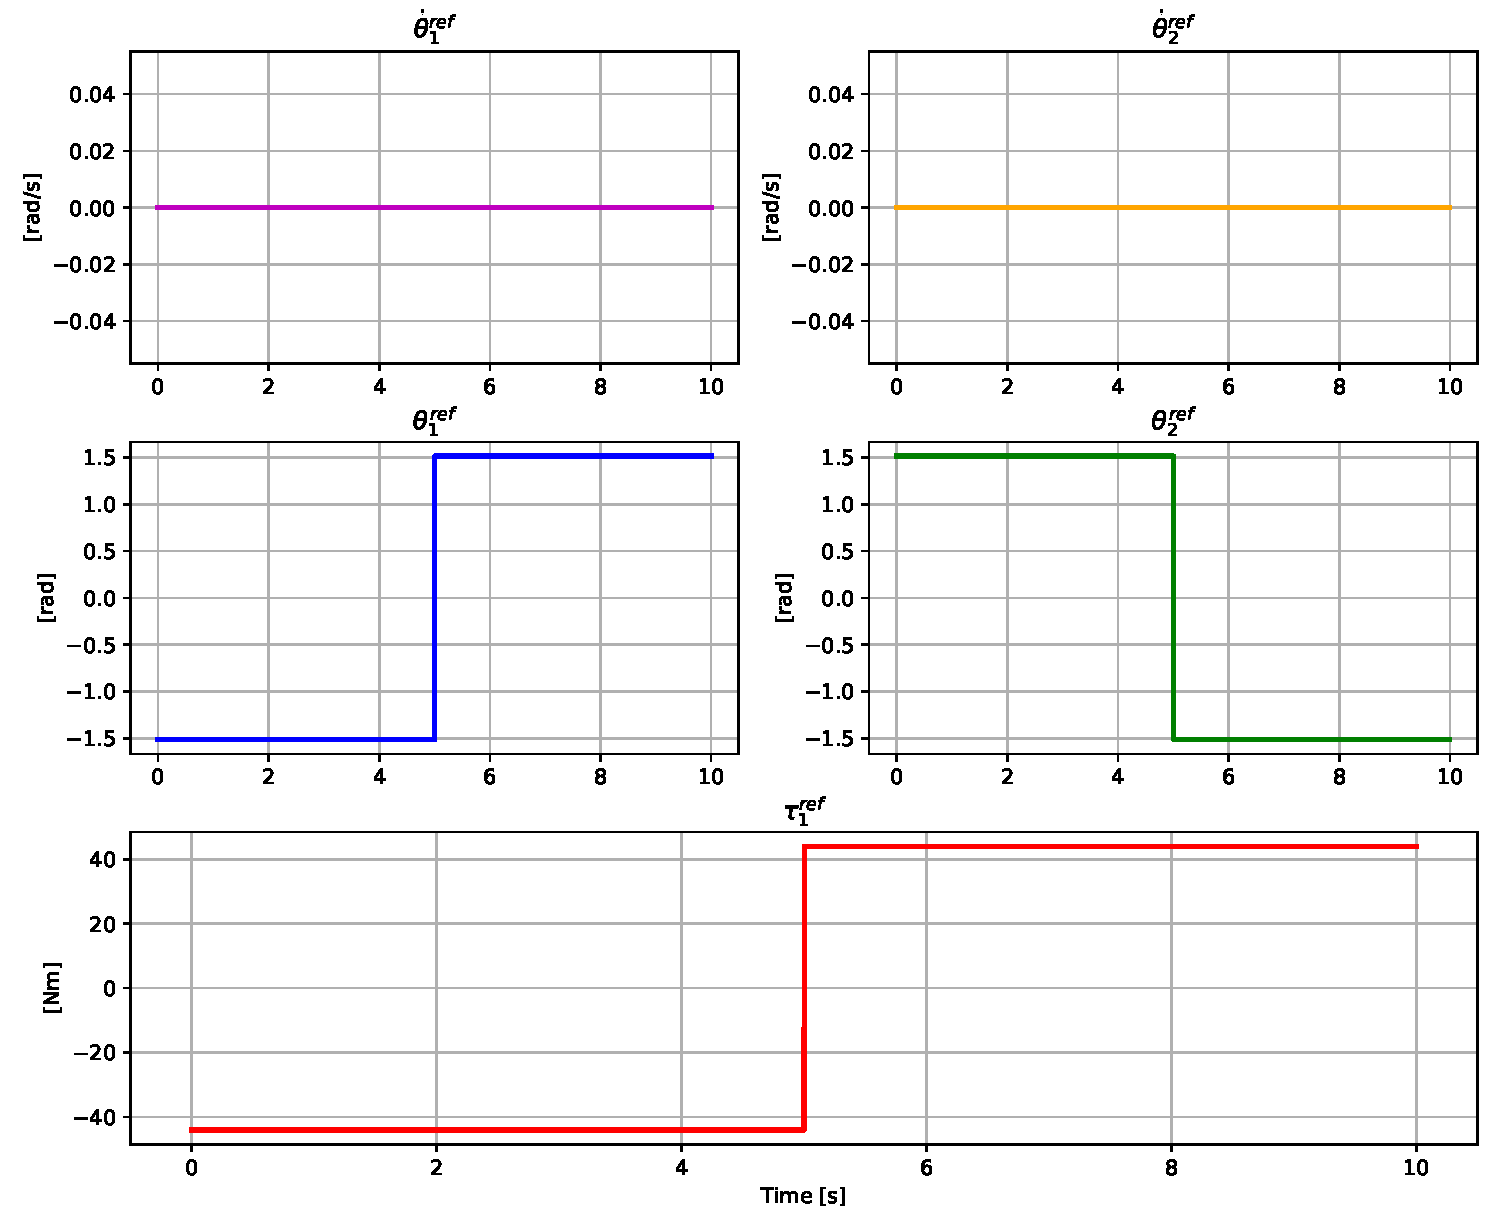
\includegraphics[width=1\linewidth]{img/1-Task1/Reference.pdf}
    \caption{Step reference curve.} %do not forget to add \cite{} inside caption if it is noy your picture
    \label{fig:step}
\end{figure}

\section{Cost Function}
The cost function is quadratic and can be written as follows:

\begin{equation}
\begin{aligned}
J(x, u) =
&\frac{1}{2} \sum_{t=0}^{T-1} \left[ (x_t - x_{\text{ref},t})^T Q_t (x_t - x_{\text{ref},t}) + (u_t - u_{\text{ref},t})^T R_t (u_t - u_{\text{ref},t}) \right] \\
&+ \frac{1}{2} (x_T - x_{\text{ref},T})^T Q_T (x_T - x_{\text{ref},T})
\end{aligned}
\label{eq:dynamics}
\end{equation}


The cost matrices are time-varying to better capture the desired behavior of the system. This approach ensures precision near the equilibrium points and allows flexibility during transitions. In particular, higher weights are assigned to emphasize accuracy at equilibrium, while lower weights are used during transitions to allow smoother adjustments. This variation is implemented in a smooth manner to ensure proper and stable control. 
For the purposes of Task 1, the cost matrices behave as follows:
\begin{figure}[htb]
    \centering
    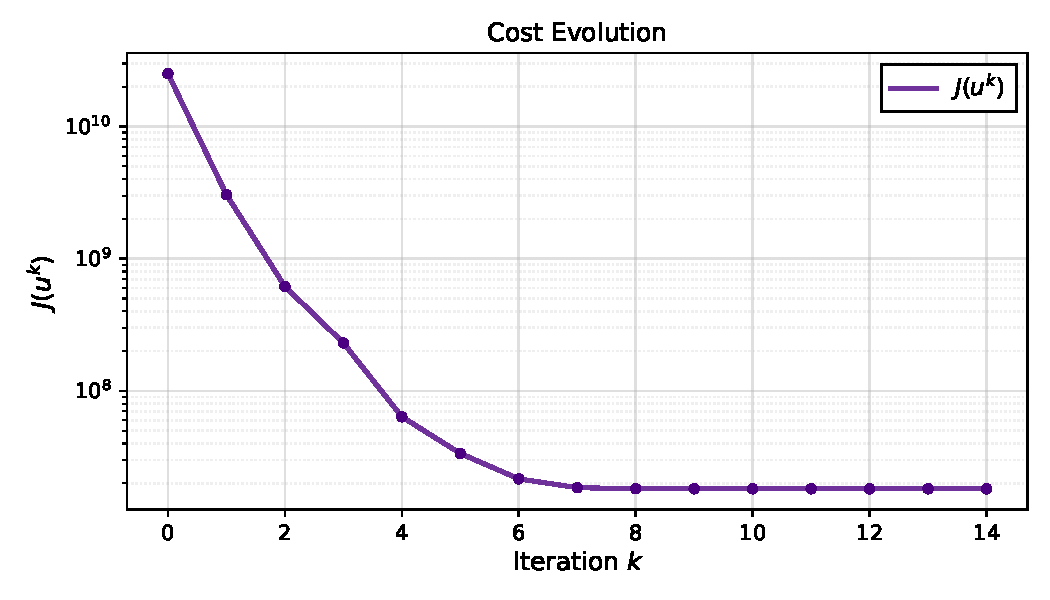
\includegraphics[width=0.8\linewidth]{img/1-Task1/cost_evolution.pdf}
    \caption{Evolution of cost matrices.}
    \label{fig:dtheta2-evolution}
\end{figure}



\section{Optimal Transition: Newton's-like Algorithm}
% - Explain the algorithm steps: initialization, descent direction computation, and parameter updates.
To achieve an optimal transition between equilibrium points, the Newton's-like algorithm for optimal control is applied in a closed-loop configuration. 
The goal is to minimize a cost function that penalizes deviations from the desired trajectory and excessive control effort.
The optimization problem states as follows:
\[min_{\mathbf{x},\mathbf{u}} \quad J(\mathbf{x},\mathbf{u})
\]
\[{s.t. }  \quad x_{t+1} = f(x_t,u_t), \quad t=0,1,...,T-1 
\]

The algorithm follows a two-step iterative procedure that involves solving the co-state equations, computing the necessary feedback gains, and updating the state-input trajectory until convergence is achieved.

In the first step, the algorithm computes the descent direction, which is essential to reduce the cost function. This involves evaluating the following terms:

\[
\nabla_1 f_t(x_t^t, u_t^t) \quad \nabla_2 f_t(x_t^t, u_t^t) \quad \nabla_1 \ell_t(x_t^t, u_t^t) \quad \nabla_2 \ell_t(x_t^t, u_t^t) \quad \nabla \ell_T(x_T^T)
\]

Once these gradients are evaluated, the co-state equations are solved backward in time, starting from \( \nabla \ell_T(x_T^T) \). The goal is to calculate the matrices \( Q_t^k \), \( R_t^k \), \( S_t^k \), and \( Q_T^k \), which are essential to obtain the feedback control law. The feedback gains \( K_t^k \) and \( \sigma_t^k \) are then computed for all time steps from \( t = 0 \) to \( t = T-1 \) by solving the optimal control problem in the backward direction.

The optimal solution of the problem reads
\begin{align*}
\Delta u_t^*      & = K_t^* \Delta x_t^* + \sigma_t^* \quad \quad \quad \quad t = 0, \ldots, T-1, \\
\Delta x_{t+1}^*  & = A_t \Delta x_t^* + B_t \Delta u_t^*,
\end{align*}
where
\begin{align*}
K_t^* & = -(R_t + B_t^\top P_{t+1} B_t)^{-1}(S_t + B_t^\top P_{t+1} A_t), \\
\sigma_t^* & = -(R_t + B_t^\top P_{t+1} B_t)^{-1}(r_t + B_t^\top p_{t+1} + B_t^\top P_{t+1} c_t), \\
p_t & = q_t + A_t^\top p_{t+1} + A_t^\top P_{t+1} c_t - K_t^{*\top} \left( R_t + B_t^\top P_{t+1} B_t \right) \sigma_t^*, \\
P_t & = Q_t + A_t^\top P_{t+1} A_t - K_t^{*\top} \left( R_t + B_t^\top P_{t+1} B_t \right) K_t^*,
\end{align*}
with \(p_T = q_T\) and \(P_T = Q_T\).
\\

The second step of the algorithm involves using the computed feedback gains to update the state and control trajectories. This is done by applying the feedback control law:

\[u^{k+1}_t = u^k_t + K^k_t \left(x^{k+1}_t - x^k_t\right) + \gamma^k \sigma^k_t
\]
Additionally, forward integration of the system dynamics is performed for all \( t = 0, \dots, T-1 \) to obtain the new trajectory. This is done by solving the system of equations:

\[x_{t+1}^{k+1} = f_t(x_t^{k+1}, u_t^{k+1})
\]
% - Highlight the role of the Armijo rule in ensuring convergence.
\[ \]

To ensure convergence and prevent overly large updates that may destabilize the trajectory, a step-size selection rule is used, such as the Armijo rule. This rule adjusts the step size based on the reduction of the cost function at each iteration, ensuring that each new trajectory results in a decrease in the overall cost.
% - Discuss parameter choices and practical considerations.

%\newpage
%\section{Plots of Generated Optimal Trajectory (I)}
%\begin{figure}[htb]
%    \centering
%    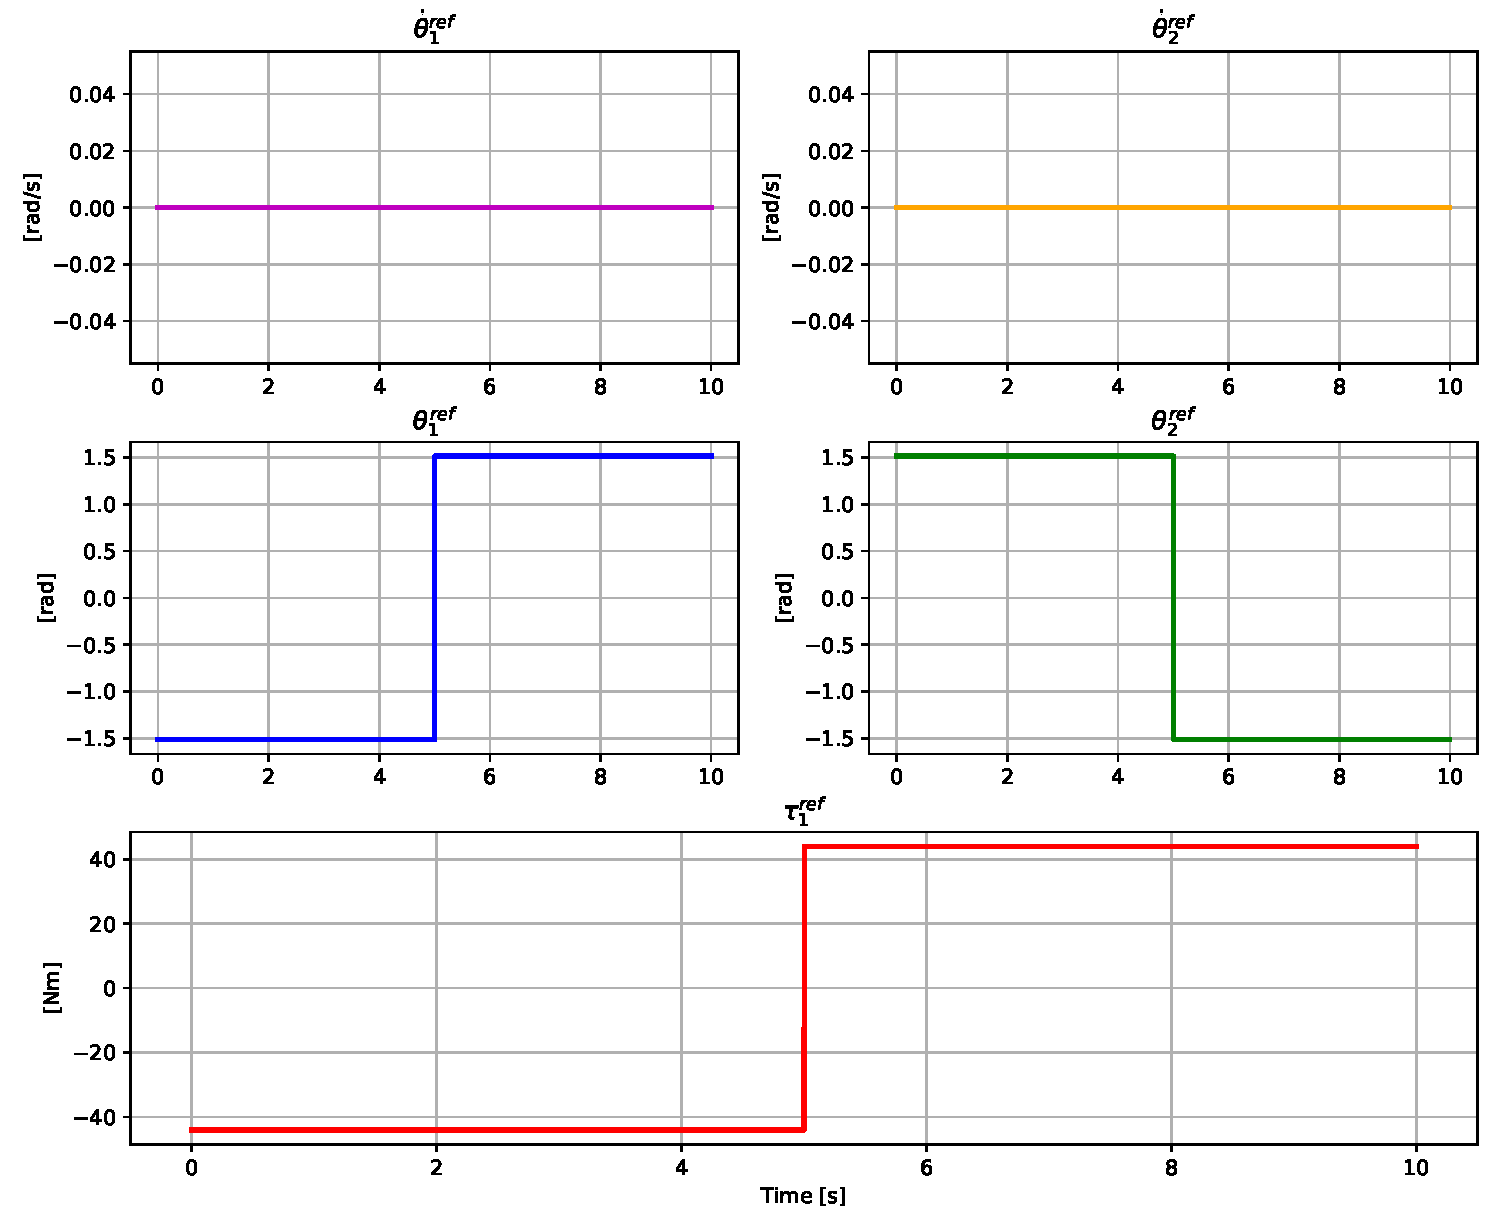
\includegraphics[width=1\linewidth]{img/1-Task1/Reference.pdf}
%    \caption{Generated optimal trajectory given a step reference.} %do not forget to add \cite{} inside caption if it is noy your picture
%    \label{fig:optimal-step}
%\end{figure}
%
%\begin{figure}[htb]
%    \centering
%    % First 3 images on the first page
%    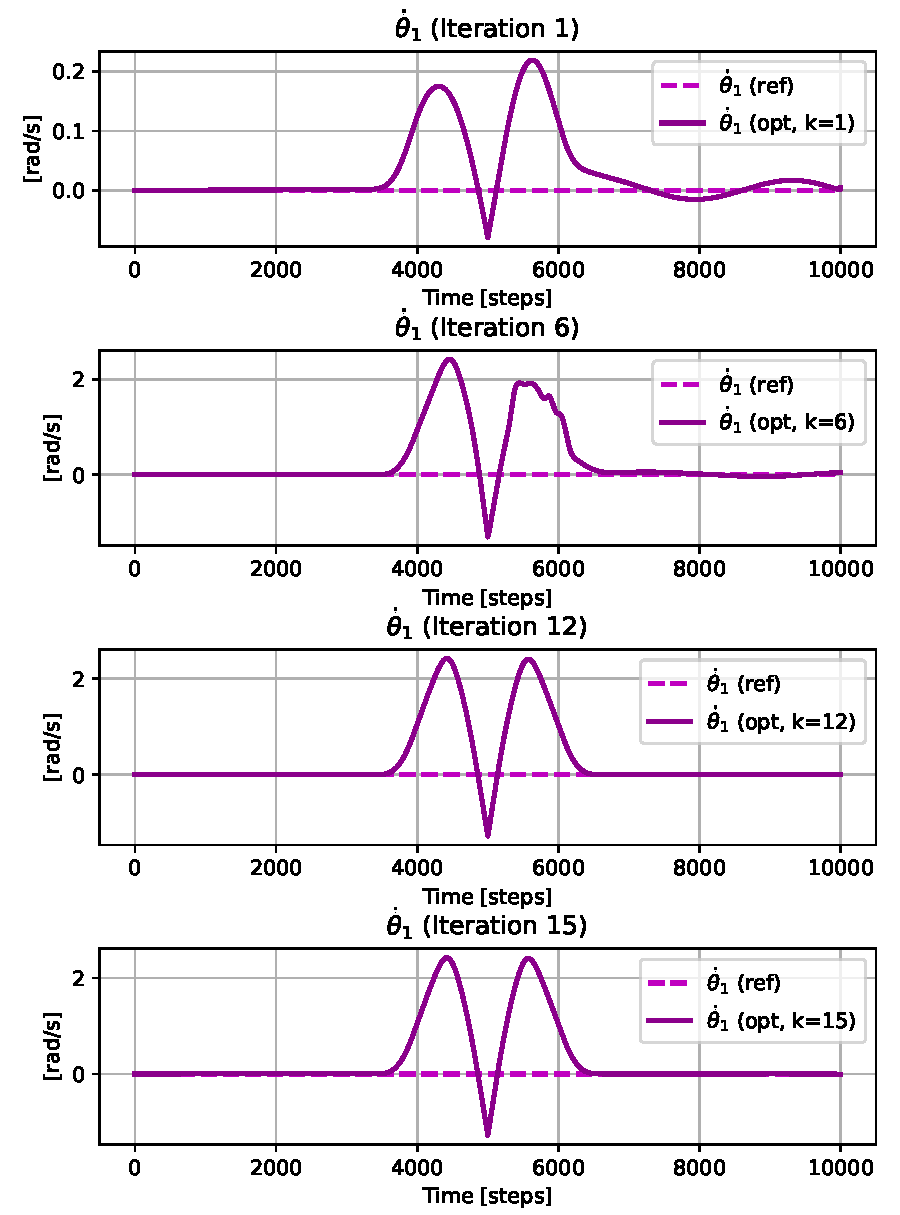
\includegraphics[width=1\linewidth]{img/1-Task1/th1dot_evolution.pdf}
%    \caption{Evolution of $d\theta_1$.}
%    \label{fig:dtheta1-evolution}
%\end{figure}
%    
%\begin{figure}[htb]
%    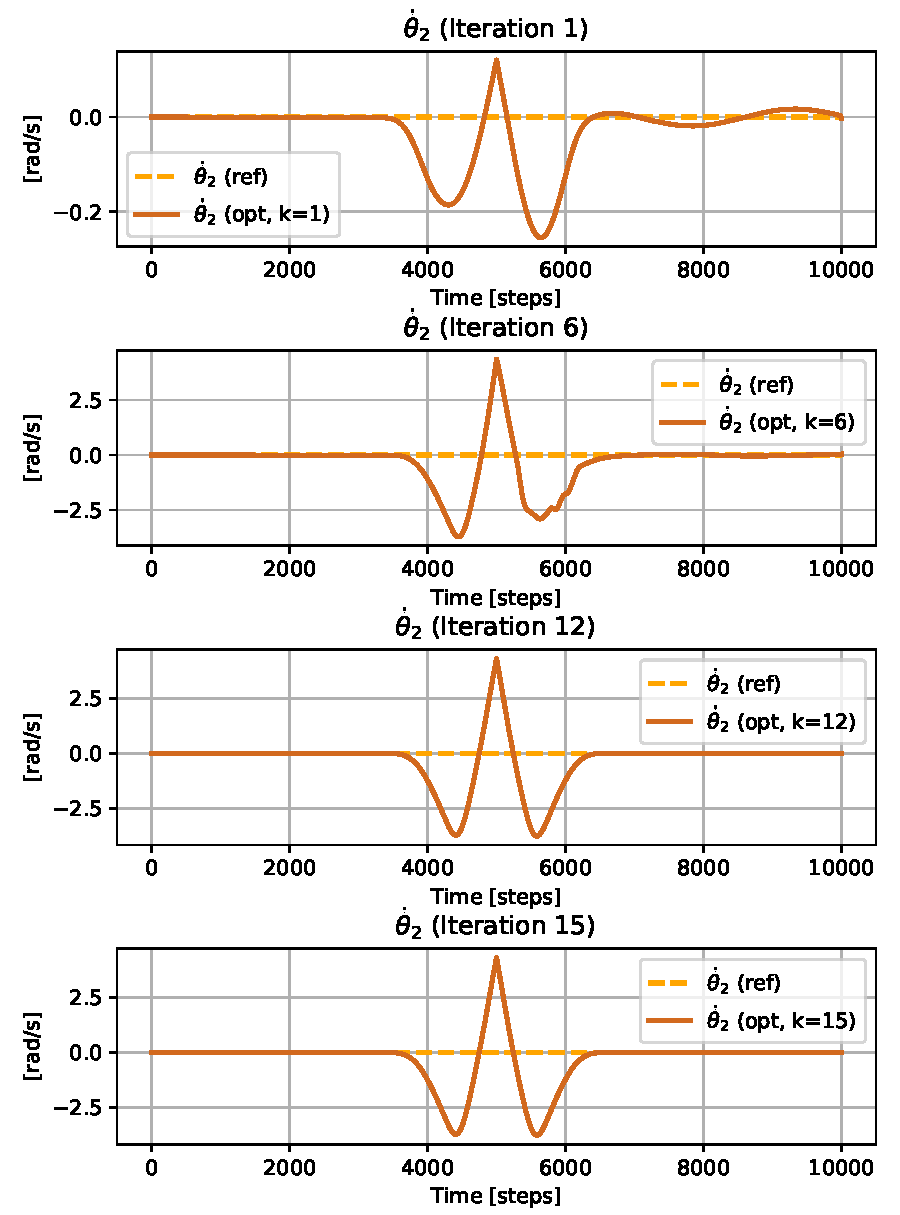
\includegraphics[width=1\linewidth]{img/1-Task1/th2dot_evolution.pdf}
%    \caption{Evolution of $d\theta_2$.}
%    \label{fig:dtheta2-evolution}
%\end{figure}
%
%\begin{figure}[htb]
%    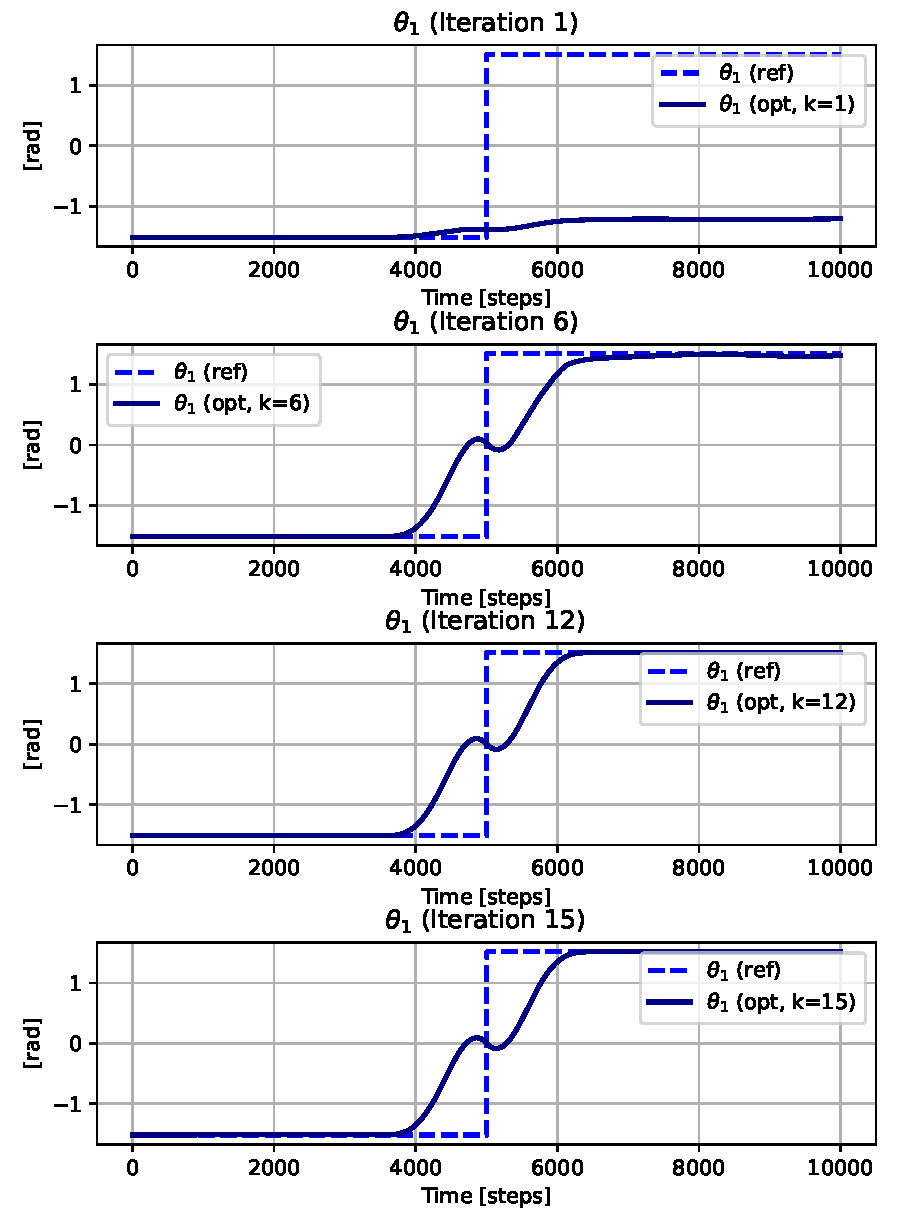
\includegraphics[width=1\linewidth]{img/1-Task1/th1_evolution.pdf}
%    \caption{Evolution of $\theta_1$.}
%    \label{fig:theta1-evolution}
%\end{figure}
%
%\begin{figure}[htb]
%    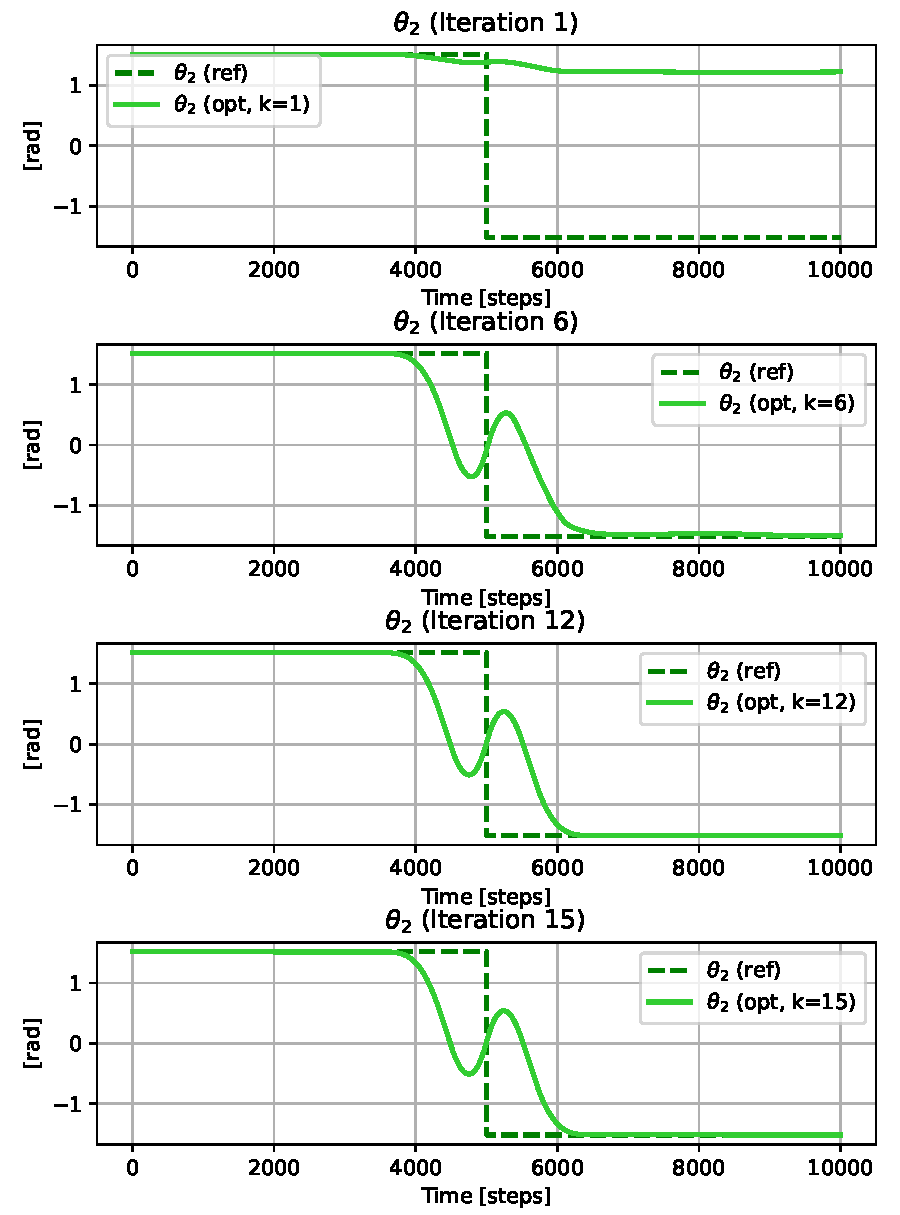
\includegraphics[width=1\linewidth]{img/1-Task1/th2_evolution.pdf}
%    \caption{Evolution of $\theta_2$.}
%    \label{fig:theta2-evolution}
%\end{figure}
%
%\begin{figure}[htb]
%    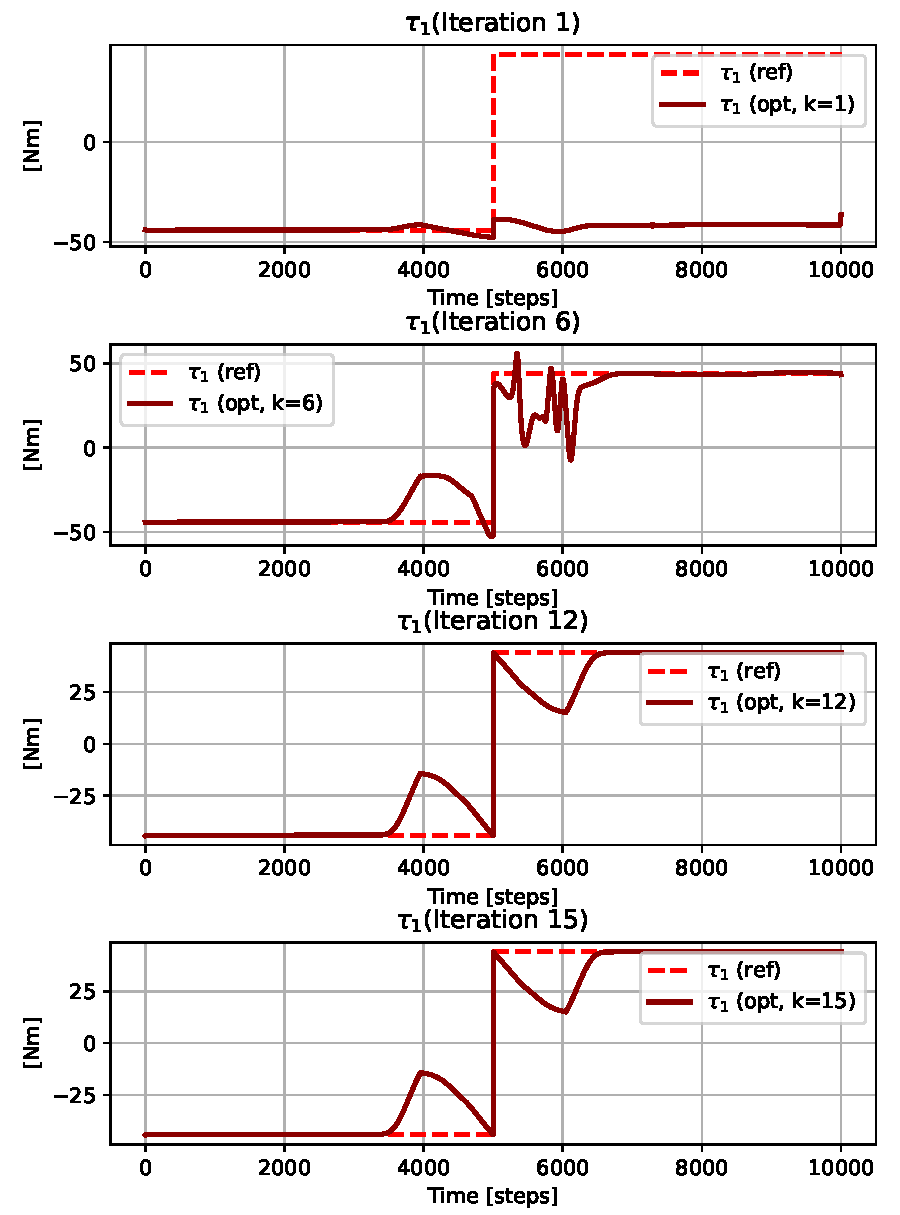
\includegraphics[width=1\linewidth]{img/1-Task1/tau_evolution.pdf}
%    \caption{Evolution of $\tau_1$.}
%    \label{fig:tau1-evolution}
%\end{figure}
%
%\begin{figure}[htb]
%    \centering
%    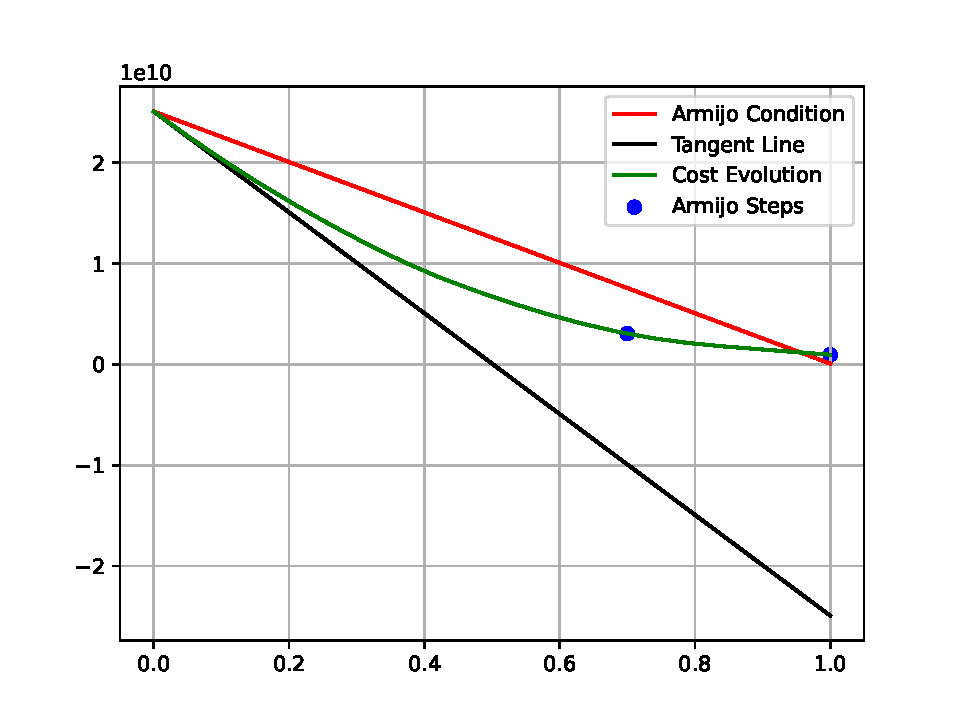
\includegraphics[width=1\linewidth]{img/1-Task1/Armijo_iter_1.pdf}
%    \caption{Armijo step-size selection: iteration 1}
%    \label{fig:armijo1}
%\end{figure}
%
%\begin{figure}[htb]
%    \centering
%    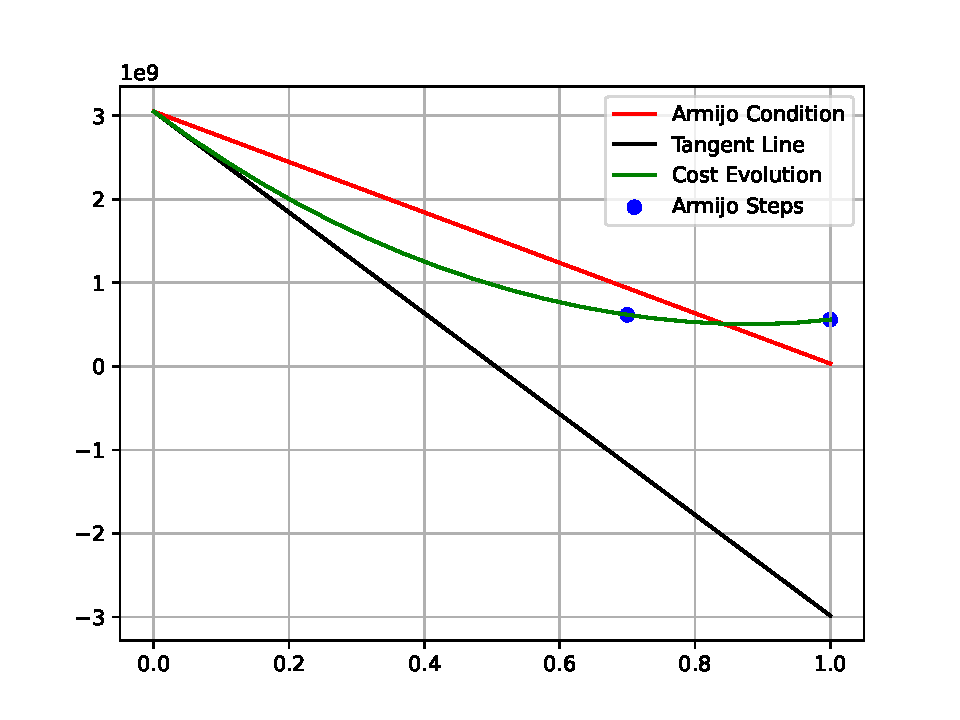
\includegraphics[width=1\linewidth]{img/1-Task1/Armijo_iter_2.pdf}
%    \caption{Armijo step-size selection: iteration 2}
%    \label{fig:armijo2}
%\end{figure}
%
%\begin{figure}[htb]
%    \centering
%    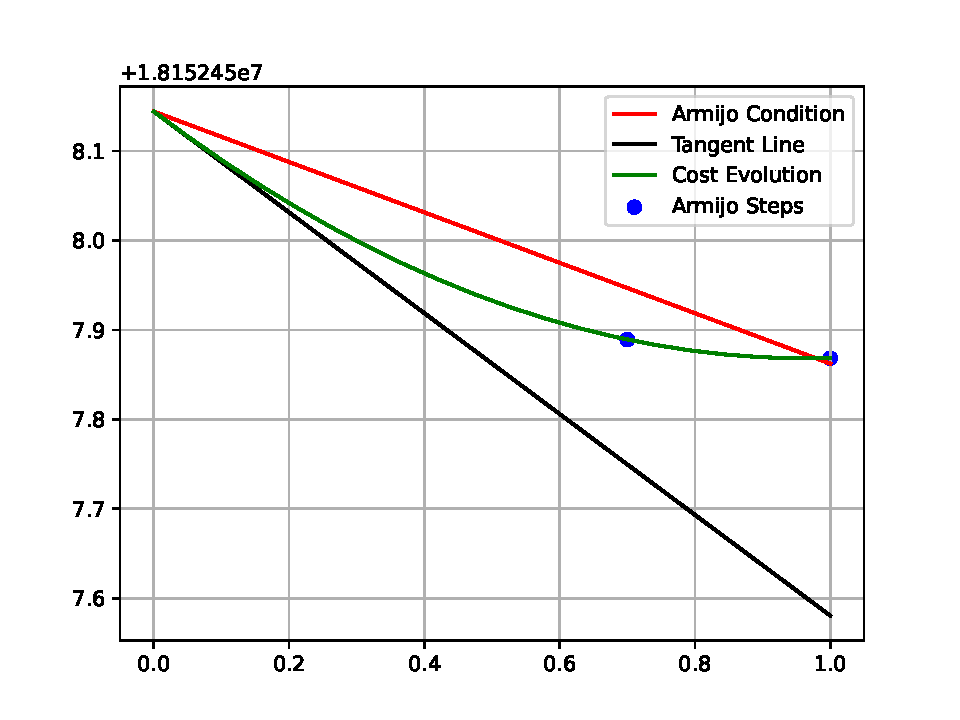
\includegraphics[width=1\linewidth]{img/1-Task1/Armijo_iter_11.pdf}
%    \caption{Armijo step-size selection: iteration 11}
%    \label{fig:armijo11}
%\end{figure}
%
%\begin{figure}[htb]
%    \centering
%    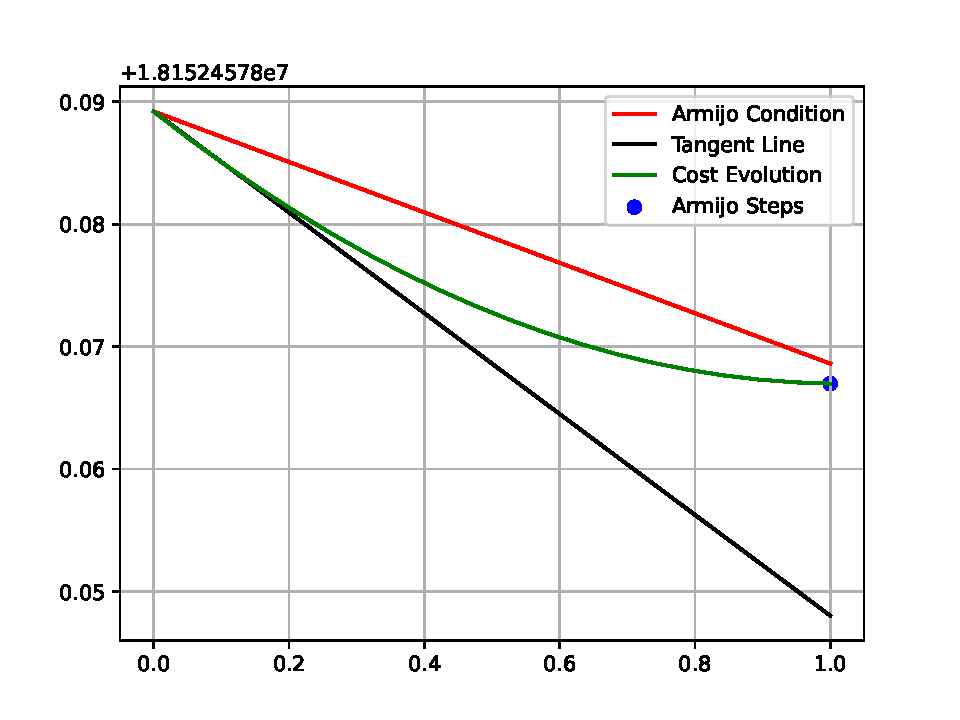
\includegraphics[width=1\linewidth]{img/1-Task1/Armijo_iter_12.pdf}
%    \caption{Armijo step-size selection: iteration 12}
%    \label{fig:armijo12}
%\end{figure}
%
%
%
%\begin{figure}[htb]
%    \centering
%    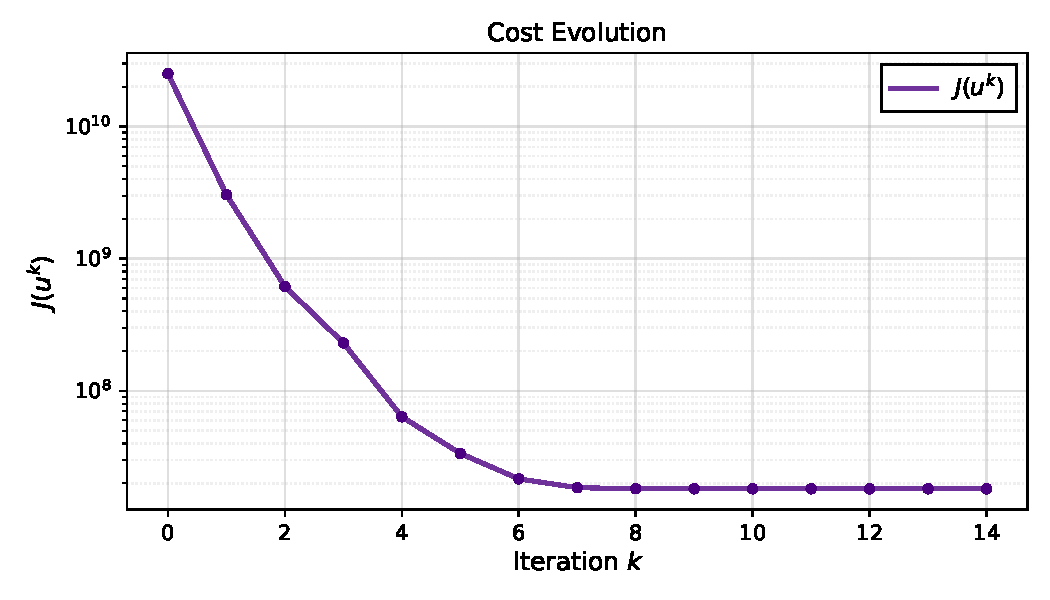
\includegraphics[width=1\linewidth]{img/1-Task1/cost_evolution.pdf}
%    \caption{Cost evolution}
%    \label{fig:t1_costevo}
%\end{figure}
%
%\begin{figure}[htb]
%    \centering
%    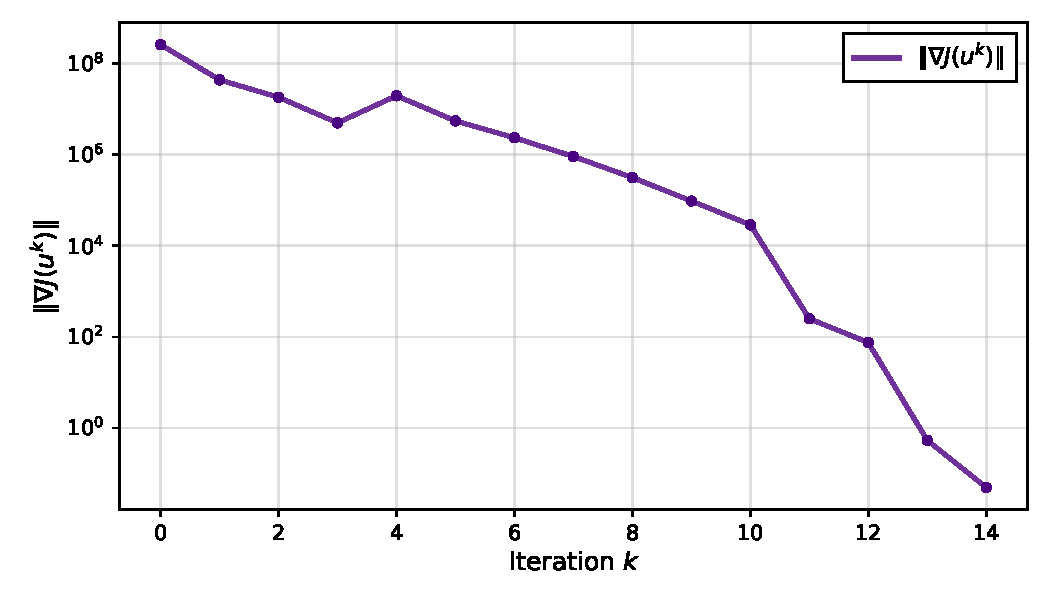
\includegraphics[width=1\linewidth]{img/1-Task1/grad_j_norm.pdf}
%    \caption{Cost gradient norm evolution}
%    \label{fig:t1_gradj}
%\end{figure}
%
%\begin{figure}[htb]
%    \centering
%    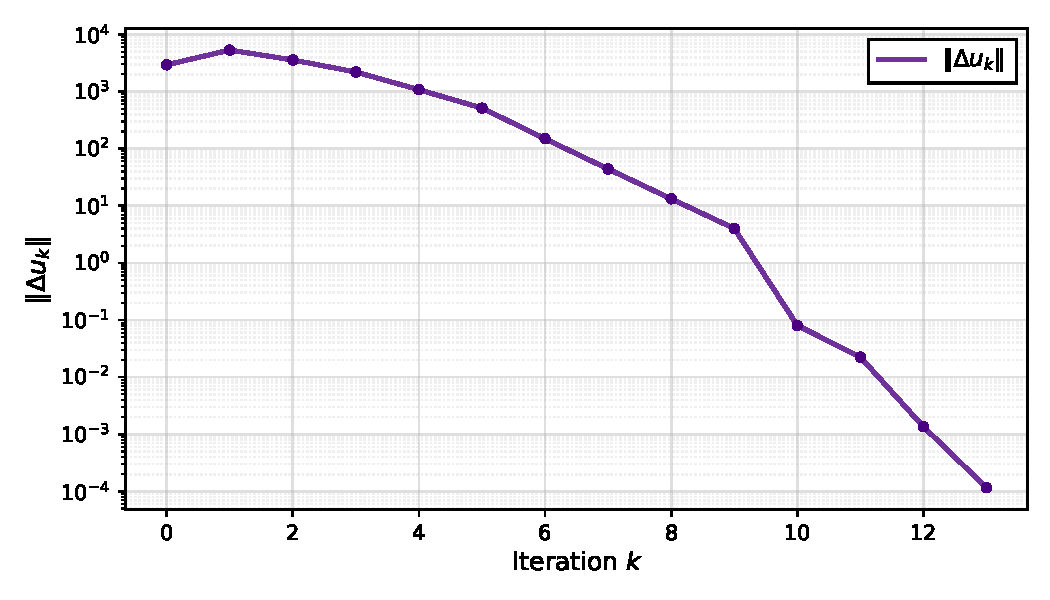
\includegraphics[width=1\linewidth]{img/1-Task1/delta_u_norm.pdf}
%    \caption{Evolution of $||\Delta u_k||$}
%    \label{fig:t1_deu}
%\end{figure}
%
%
%\newpage
%\section{Constant Cost Matrices Scenario}
%For the sake of completeness, a case with constant cost matrices has also been considered. The cost has also been normalized. The following Cost Matrices have been adopted:
%\begin{equation}
%Q_t = Q_T
%=
%\begin{bmatrix}
%    10 & 0 & 0 & 0\\
%    0 & 10 & 0 & 0\\
%    0 & 0 & 10 & 0\\
%    0 & 0 & 0  &10\\
%\end{bmatrix}
%\label{eq:CosntantQ}
%\end{equation}
%
%\begin{equation}
%R_t = 
%\begin{bmatrix}
%    0.3 & 0 & 0 & 0\\
%    0 & 0.3 & 0 & 0\\
%    0 & 0 & 0.3 & 0\\
%    0 & 0 & 0 & 0.3\\
%\end{bmatrix}
%\label{eq:ConstantR}
%\end{equation}
%
%Here, a summary of the results is presented.
% 
%\begin{figure}[htb]
%    \centering
%    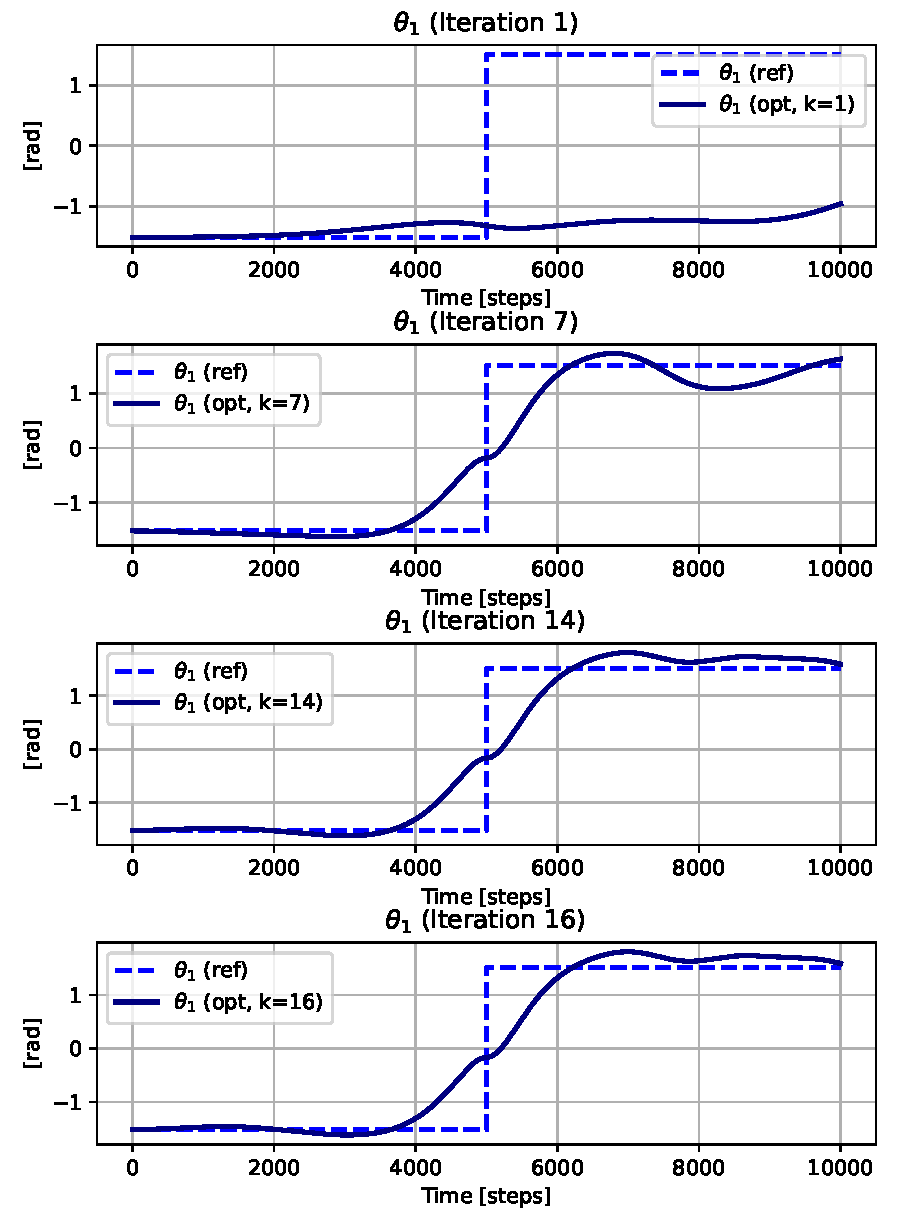
\includegraphics[width=1\linewidth]{img/1-Task1/th1_const.pdf}
%    \caption{Evolution of $\theta_1$ with constant Cost Matrices}
%    \label{fig:th1const}
%\end{figure}
%
%\begin{figure}[htb]
%    \centering
%    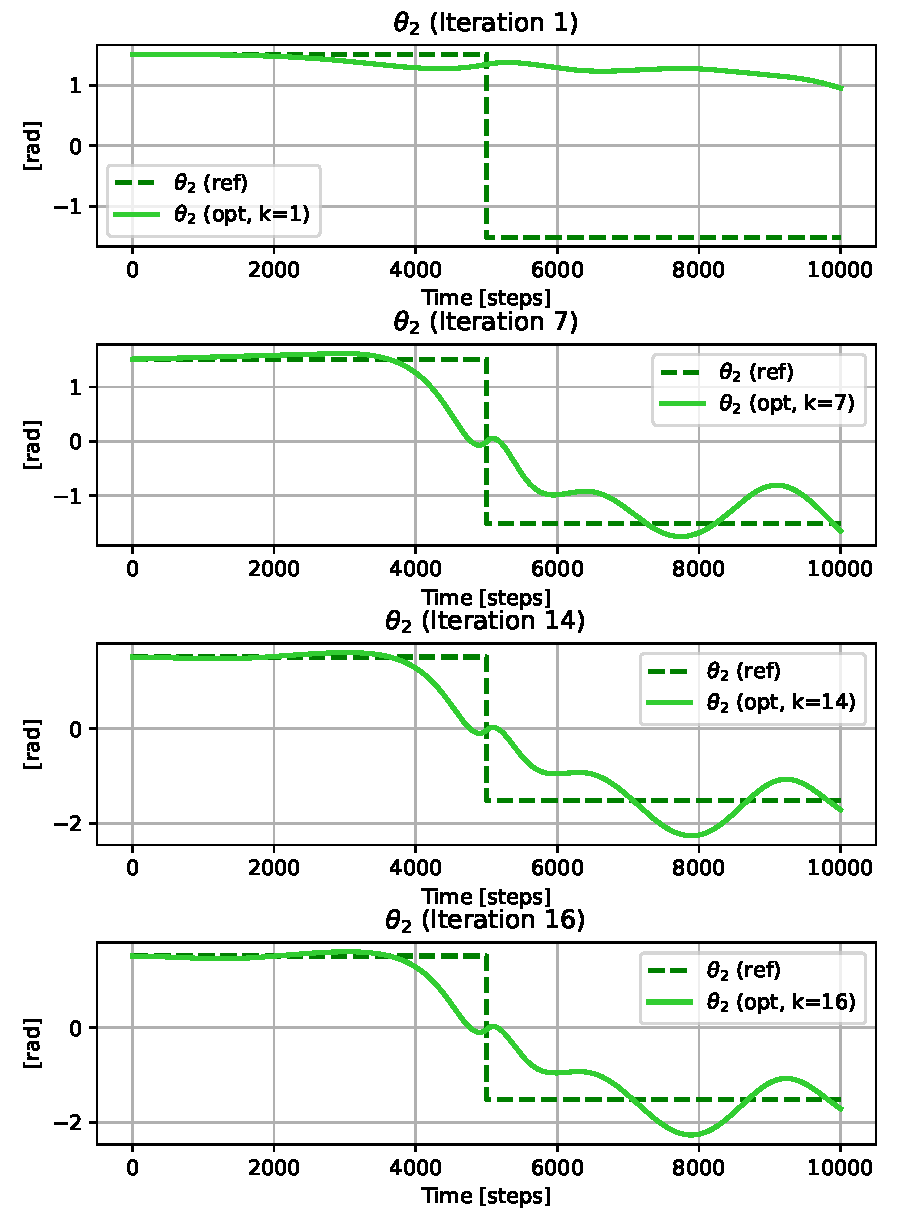
\includegraphics[width=1\linewidth]{img/1-Task1/th2_const.pdf}
%    \caption{Evolution of $\theta_2$ with constant Cost Matrices}
%    \label{fig:th2const}
%\end{figure}
%
%\begin{figure}[htb]
%    \centering
%    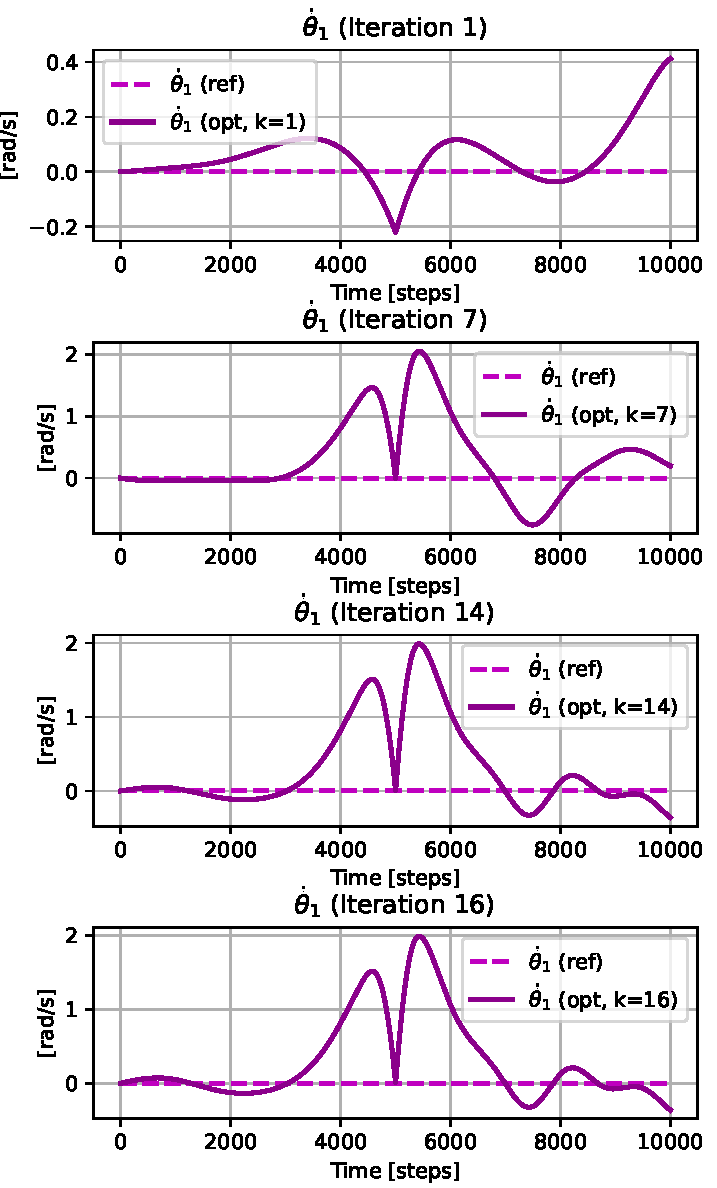
\includegraphics[width=0.9\linewidth]{img/1-Task1/th1dot_const.pdf}
%    \caption{Evolution of $\dot{\theta_1}$ with constant Cost Matrices}
%    \label{fig:th1dot_const}
%\end{figure}
%
%\begin{figure}[htb]
%    \centering
%    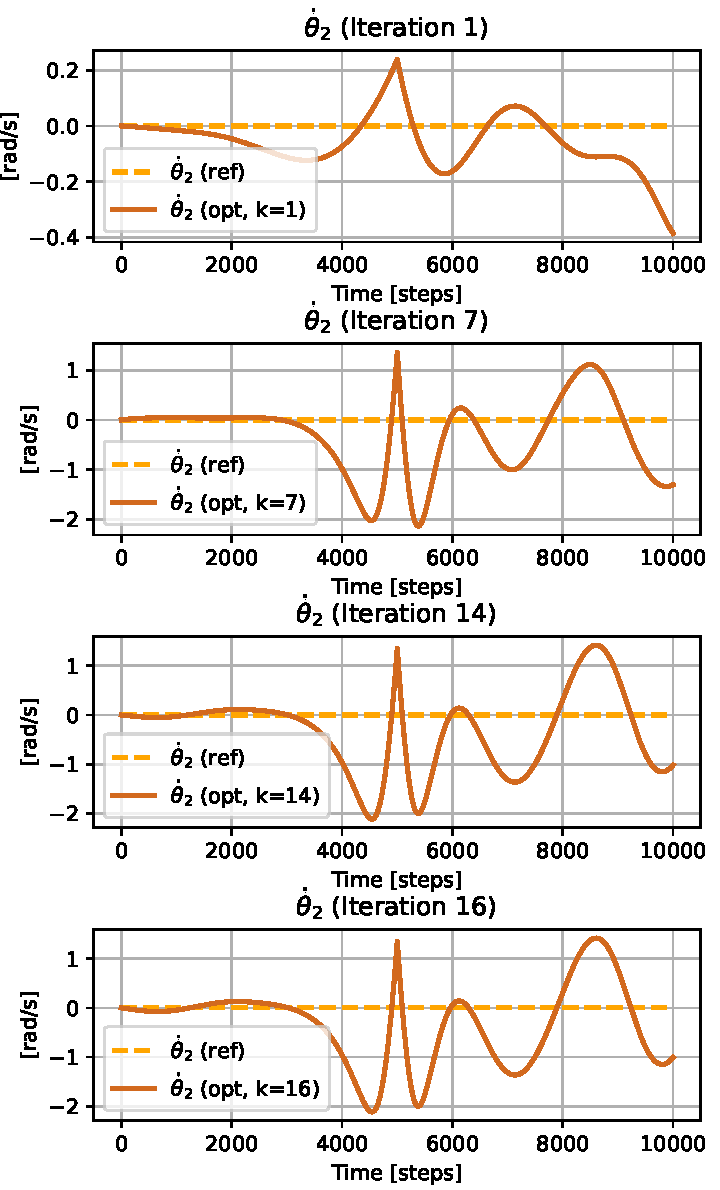
\includegraphics[width=1\linewidth]{img/1-Task1/th2dot_const.pdf}
%    \caption{Evolution of $\dot{\theta_2}$ with constant Cost Matrices}
%    \label{fig:th2_const}
%\end{figure}
%
%\begin{figure}[htb]
%    \centering
%    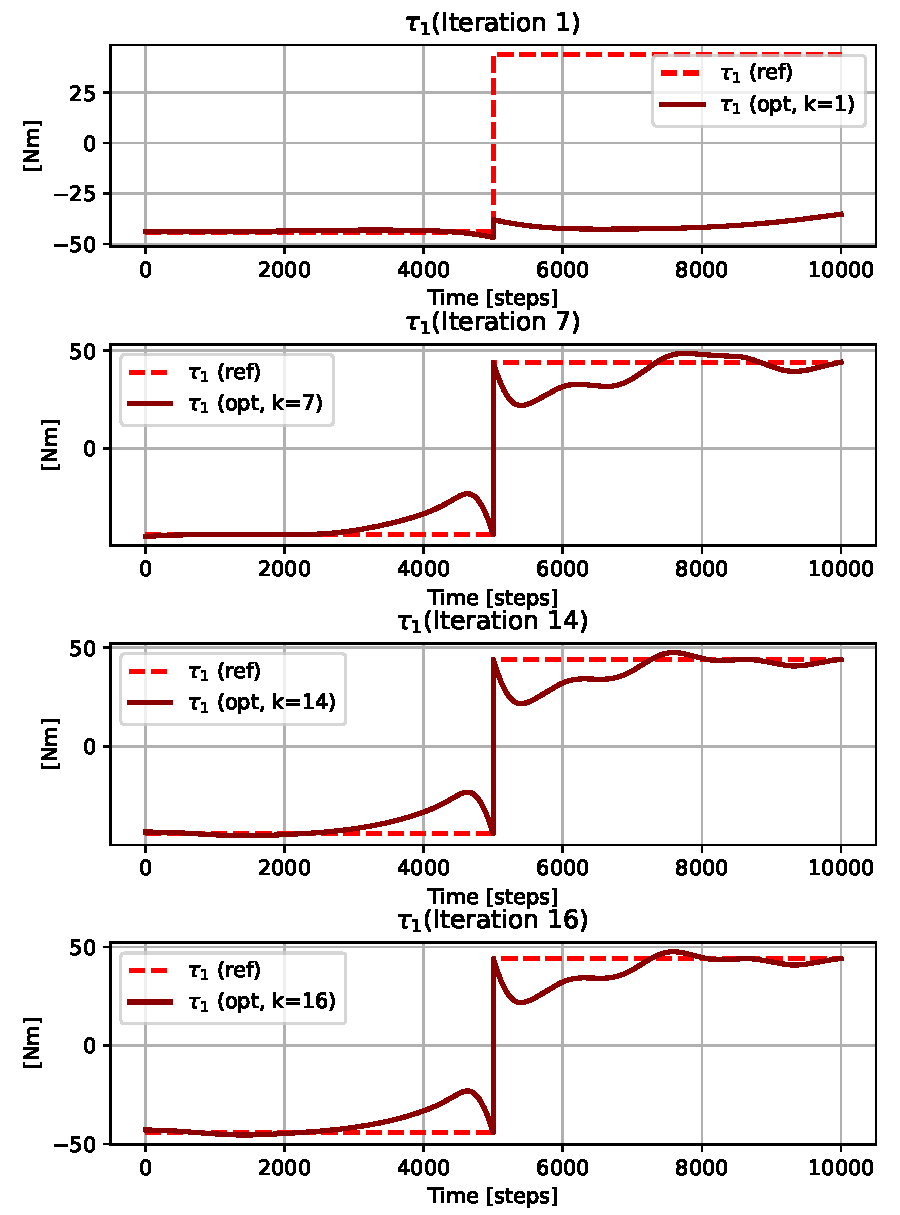
\includegraphics[width=1\linewidth]{img/1-Task1/tau1_const.pdf}
%    \caption{Evolution of $\tau$ with constant Cost Matrices}
%    \label{fig:tau_const}
%\end{figure}
%
%\begin{figure}[htb]
%    \centering
%    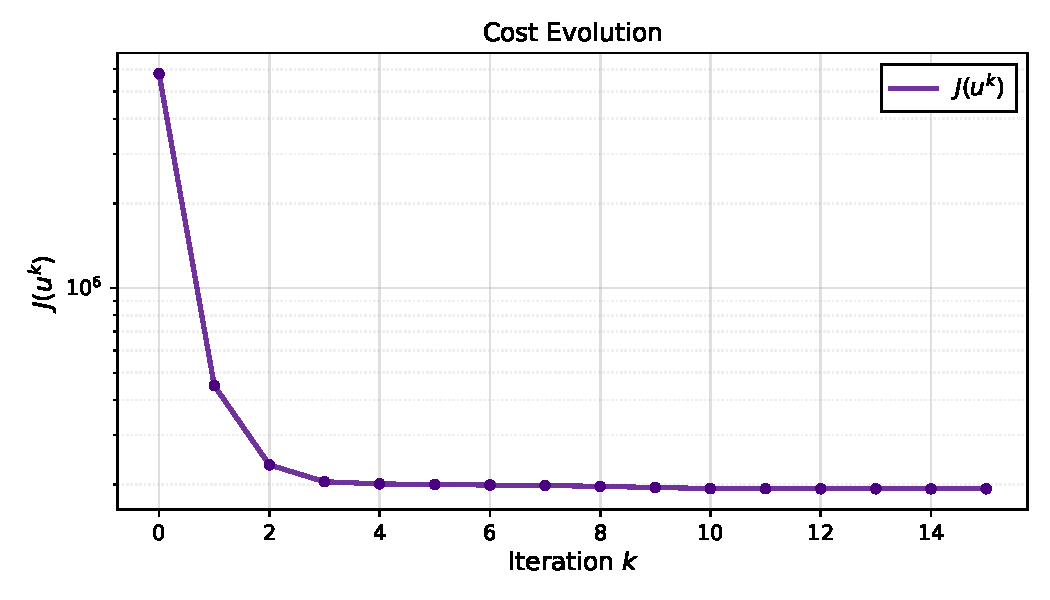
\includegraphics[width=1\linewidth]{img/1-Task1/J_const.pdf}
%    \caption{Evolution of cost function with constant Cost Matrices}
%    \label{fig:J_const}
%\end{figure}
%
%\begin{figure}[htb]
%    \centering
%    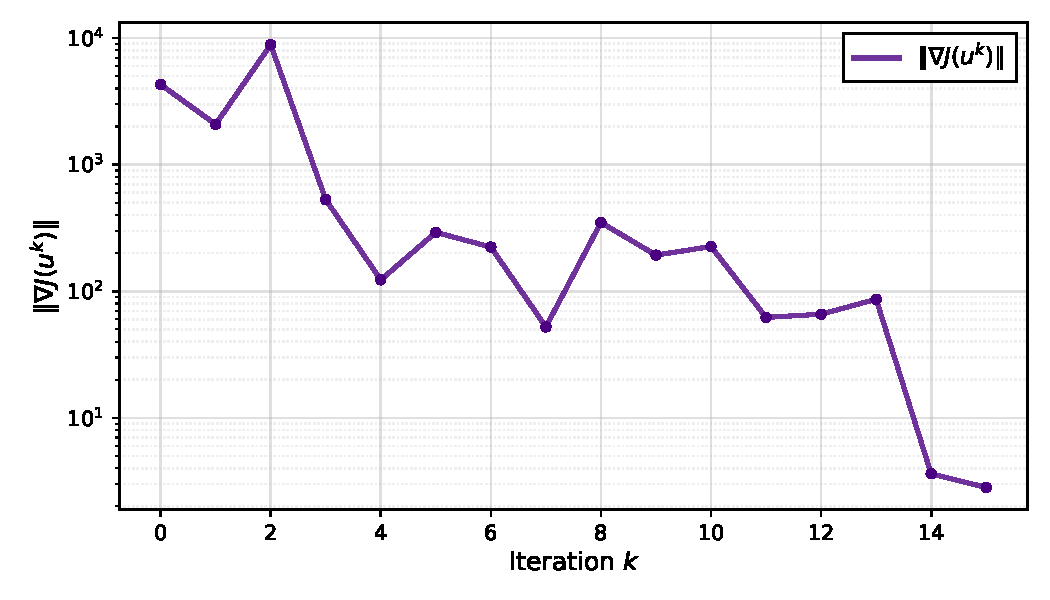
\includegraphics[width=1\linewidth]{img/1-Task1/NormJ_const.pdf}
%    \caption{Evolution of $||\nabla J(u)||$ with constant Cost Matrices}
%    \label{fig:NormJ_const}
%\end{figure}
%
%\begin{figure}[htb]
%    \centering
%    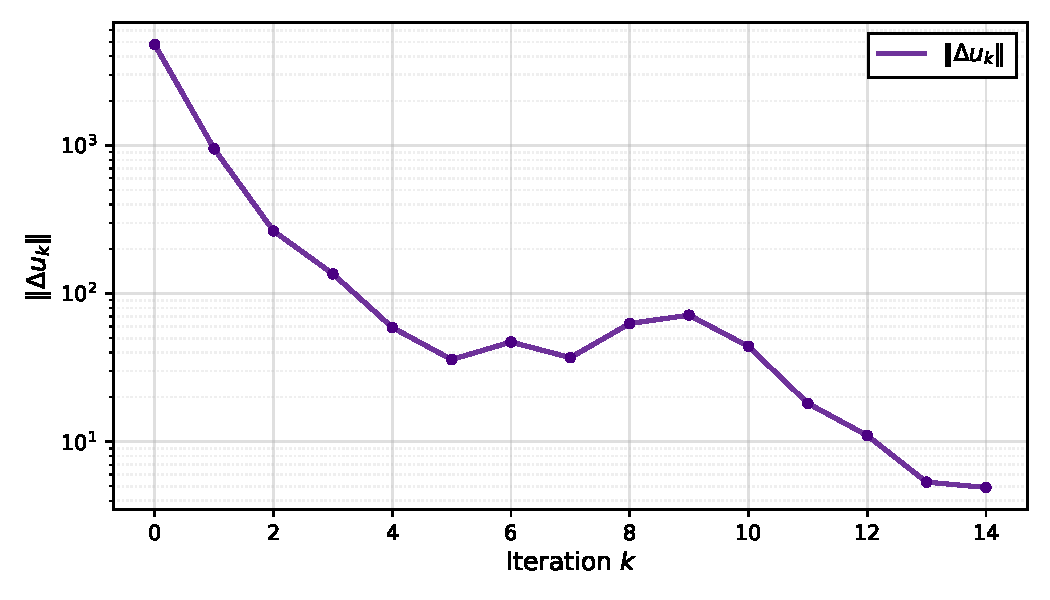
\includegraphics[width=1\linewidth]{img/1-Task1/normdu_const.pdf}
%    \caption{Evolution of $||\Delta u_k||$ with constant Cost Matrices}
%    \label{fig:normdu_const}
%\end{figure}

\newpage
\section{Plots of Generated Optimal Trajectory (I)}

\begin{figure}[htb]
    \centering
    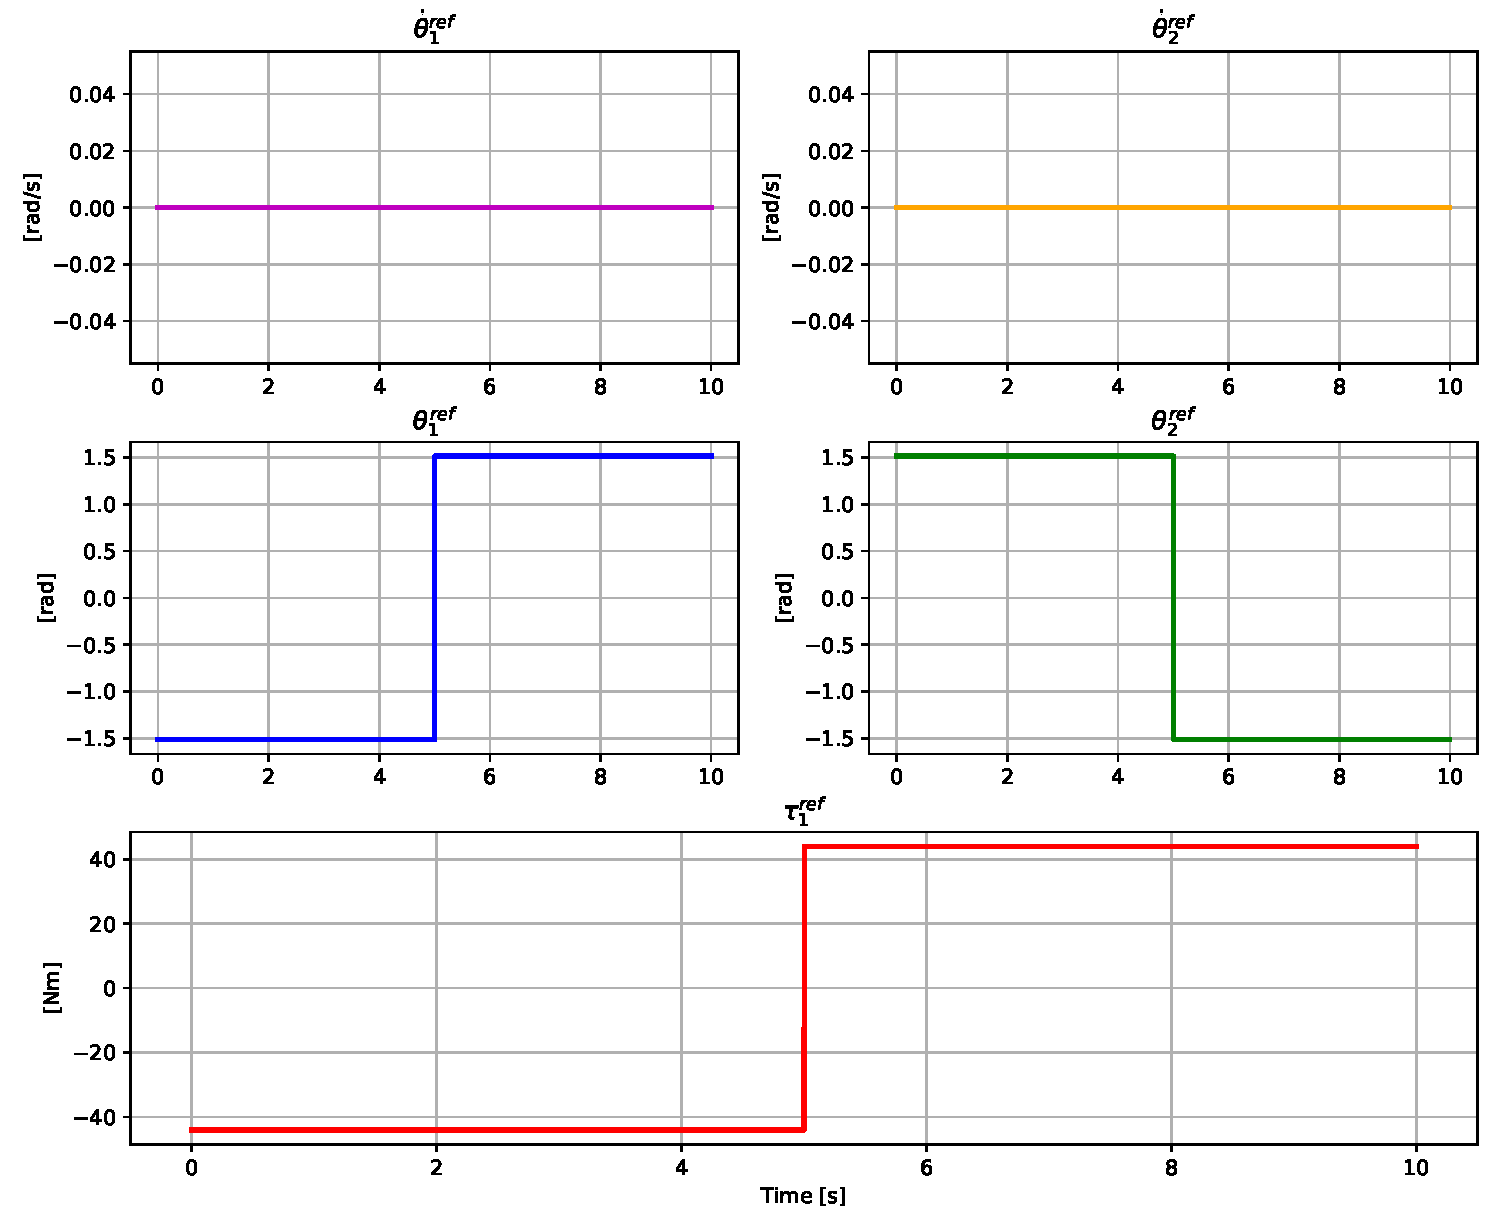
\includegraphics[width=1\linewidth]{img/1-Task1/Reference.pdf}
    \caption{Generated optimal trajectory given a step reference.}
    \label{fig:optimal-step}
\end{figure}

\begin{figure}[htb]
    \centering
    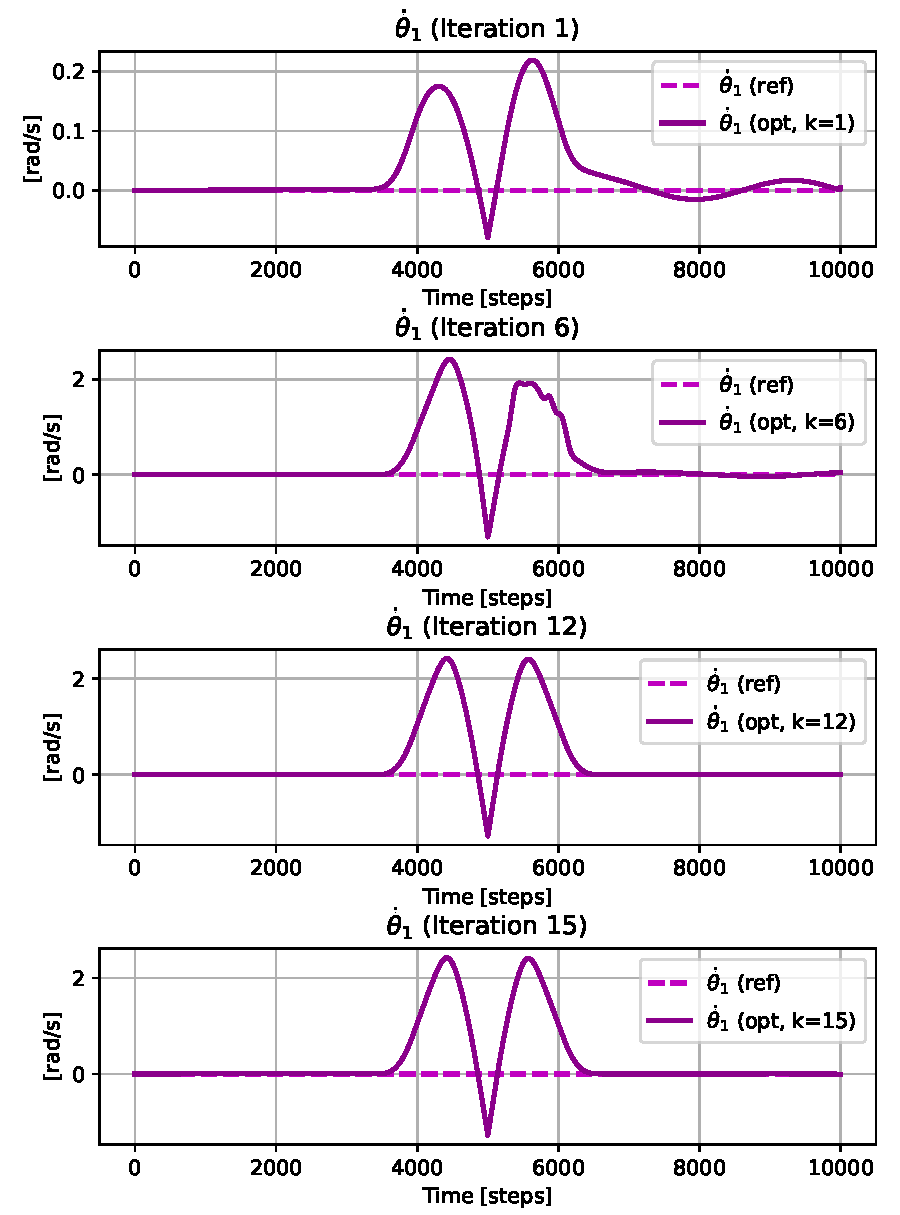
\includegraphics[width=1\linewidth]{img/1-Task1/th1dot_evolution.pdf}
    \caption{Evolution of $d\theta_1$.}
    \label{fig:dtheta1-evolution}
\end{figure}

\begin{figure}[htb]
    \centering
    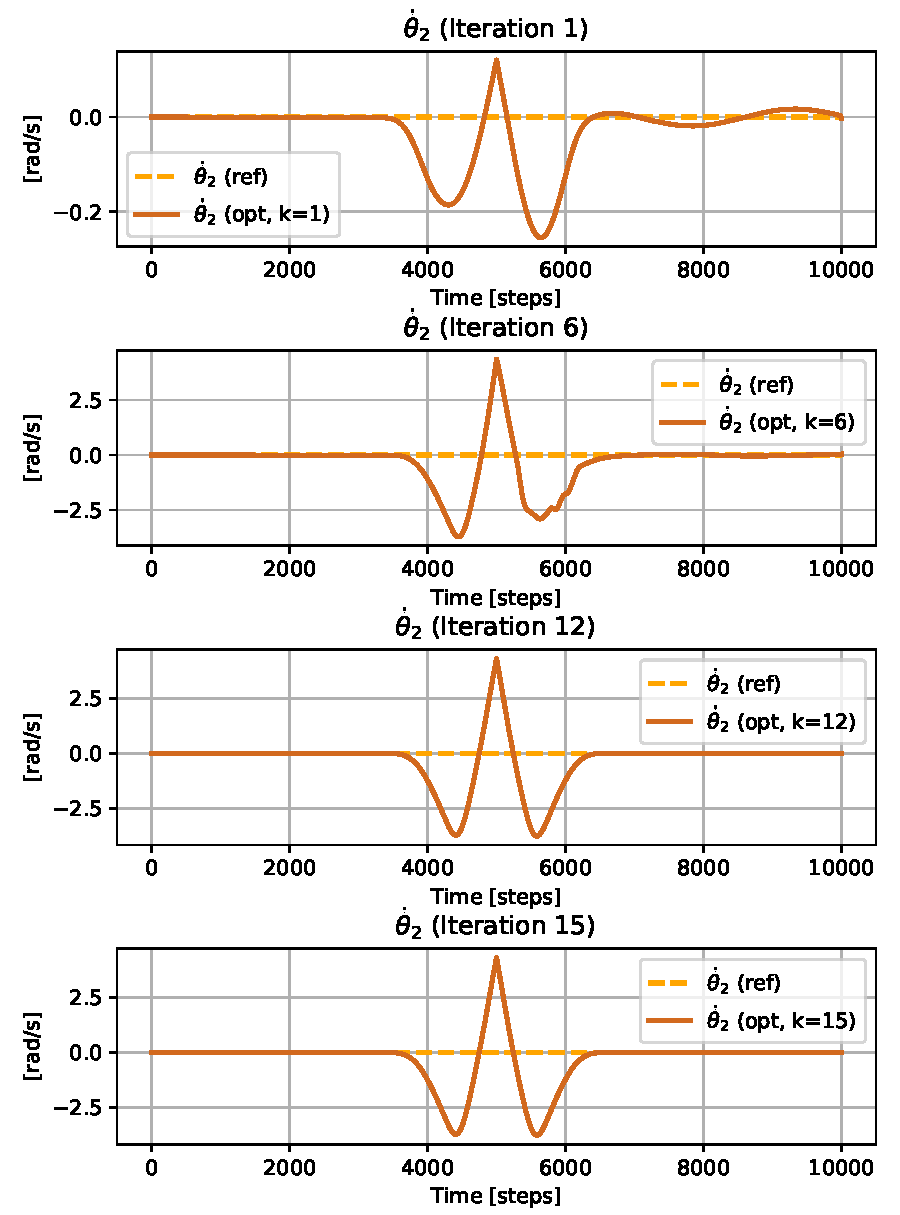
\includegraphics[width=1\linewidth]{img/1-Task1/th2dot_evolution.pdf}
    \caption{Evolution of $d\theta_2$.}
    \label{fig:dtheta2-evolution}
\end{figure}

\clearpage

\begin{figure}[htb]
    \centering
    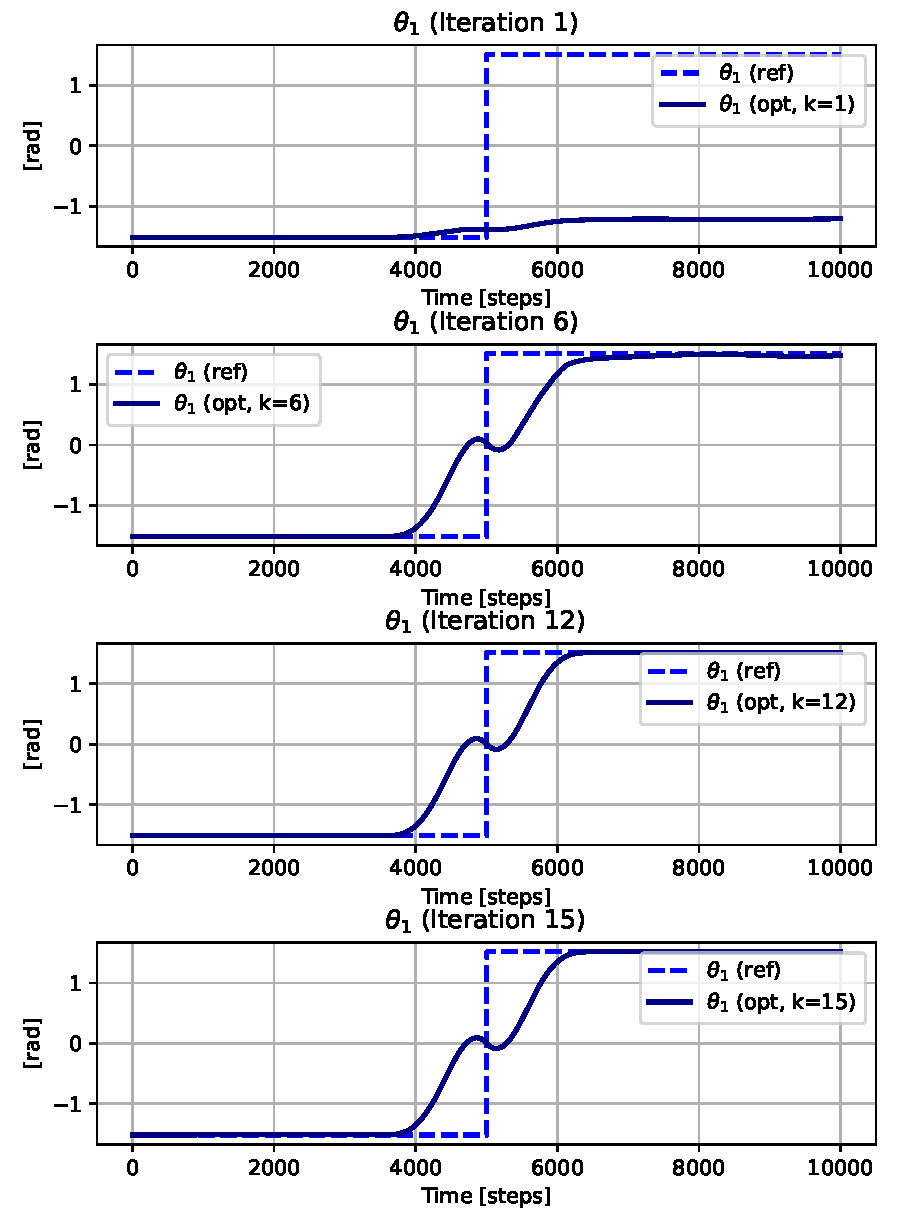
\includegraphics[width=1\linewidth]{img/1-Task1/th1_evolution.pdf}
    \caption{Evolution of $\theta_1$.}
    \label{fig:theta1-evolution}
\end{figure}

\begin{figure}[htb]
    \centering
    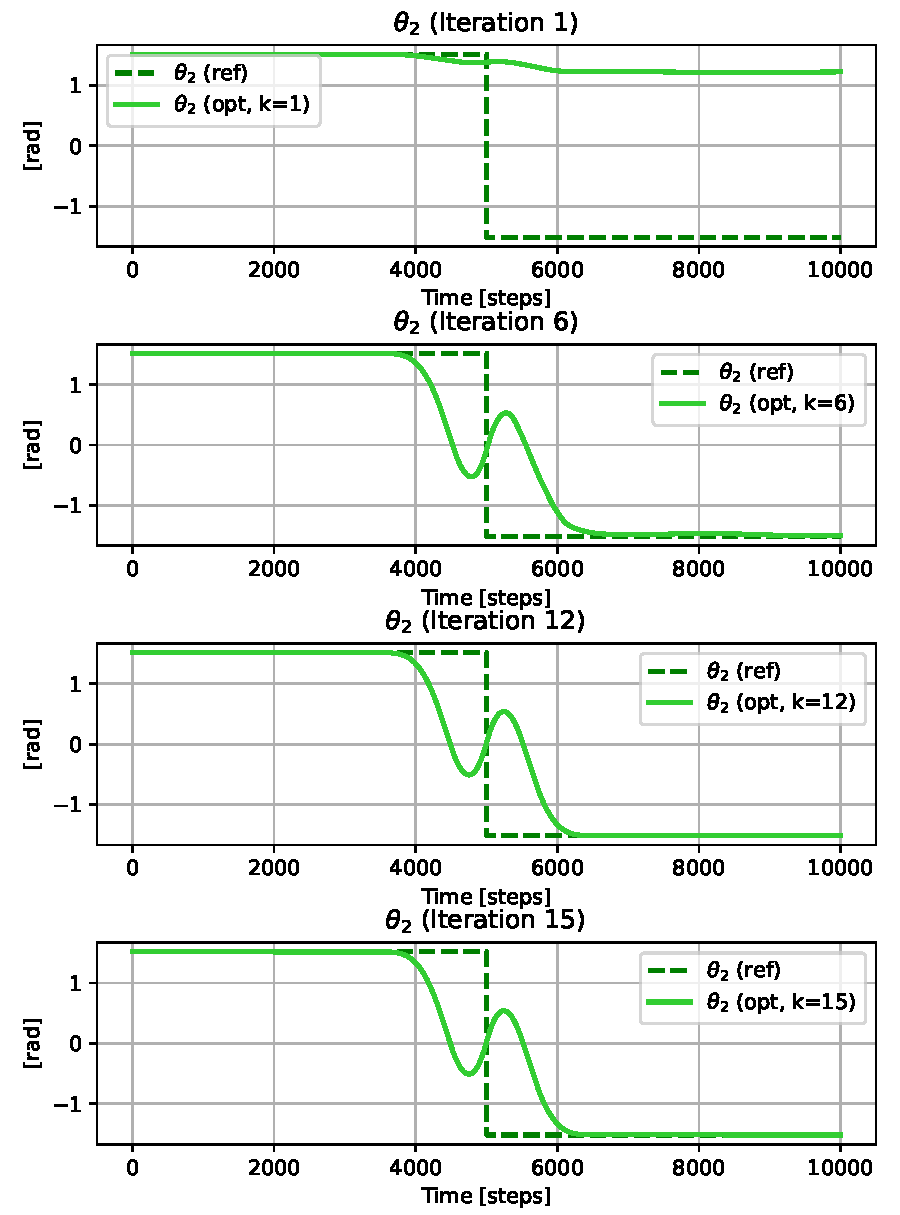
\includegraphics[width=1\linewidth]{img/1-Task1/th2_evolution.pdf}
    \caption{Evolution of $\theta_2$.}
    \label{fig:theta2-evolution}
\end{figure}

\begin{figure}[htb]
    \centering
    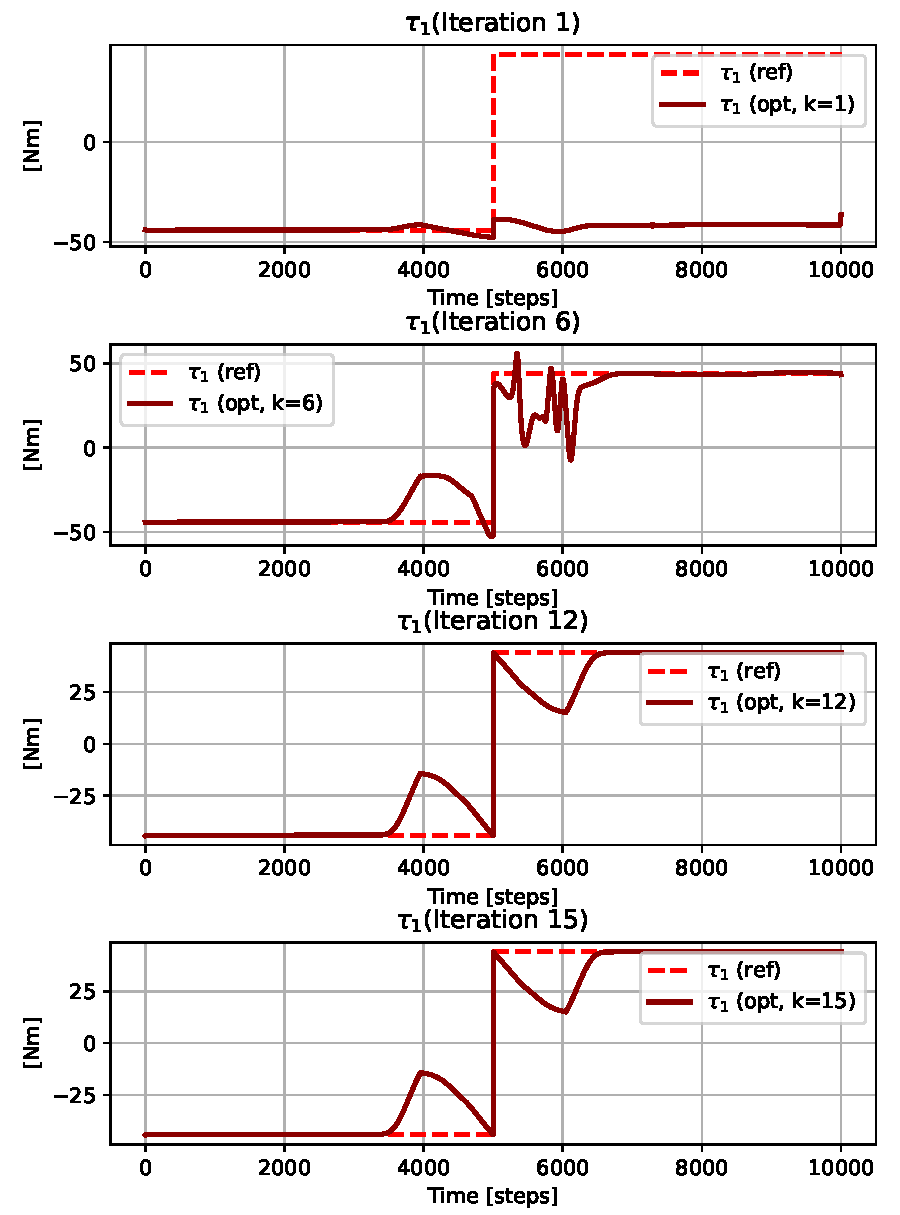
\includegraphics[width=1\linewidth]{img/1-Task1/tau_evolution.pdf}
    \caption{Evolution of $\tau_1$.}
    \label{fig:tau1-evolution}
\end{figure}

\begin{figure}[htb]
    \centering
    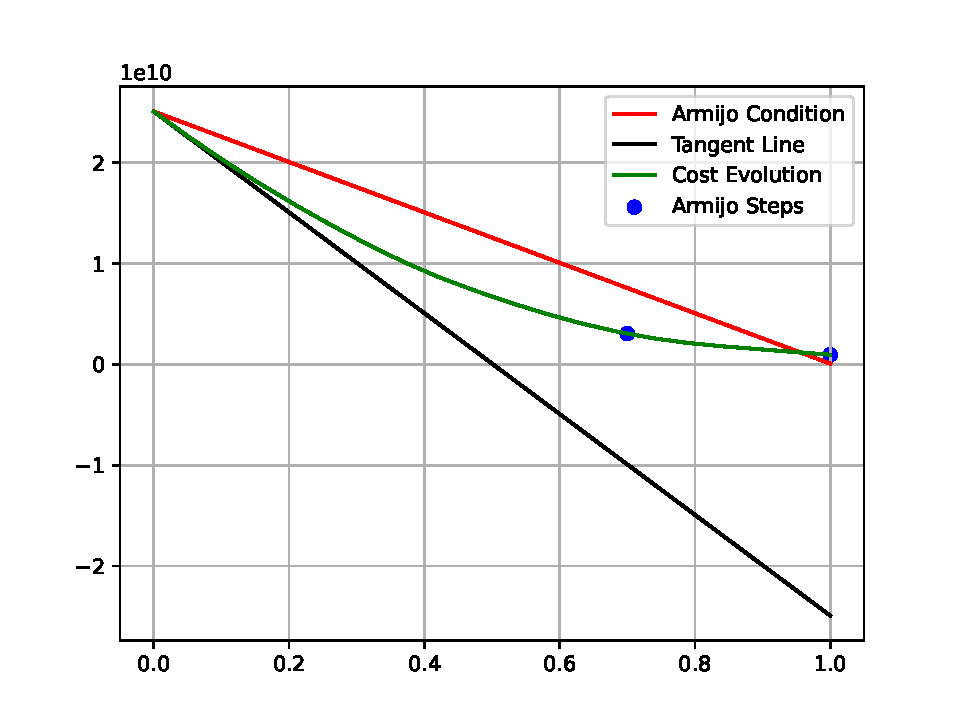
\includegraphics[width=1\linewidth]{img/1-Task1/Armijo_iter_1.pdf}
    \caption{Armijo step-size selection: iteration 1.}
    \label{fig:armijo1}
\end{figure}

\begin{figure}[htb]
    \centering
    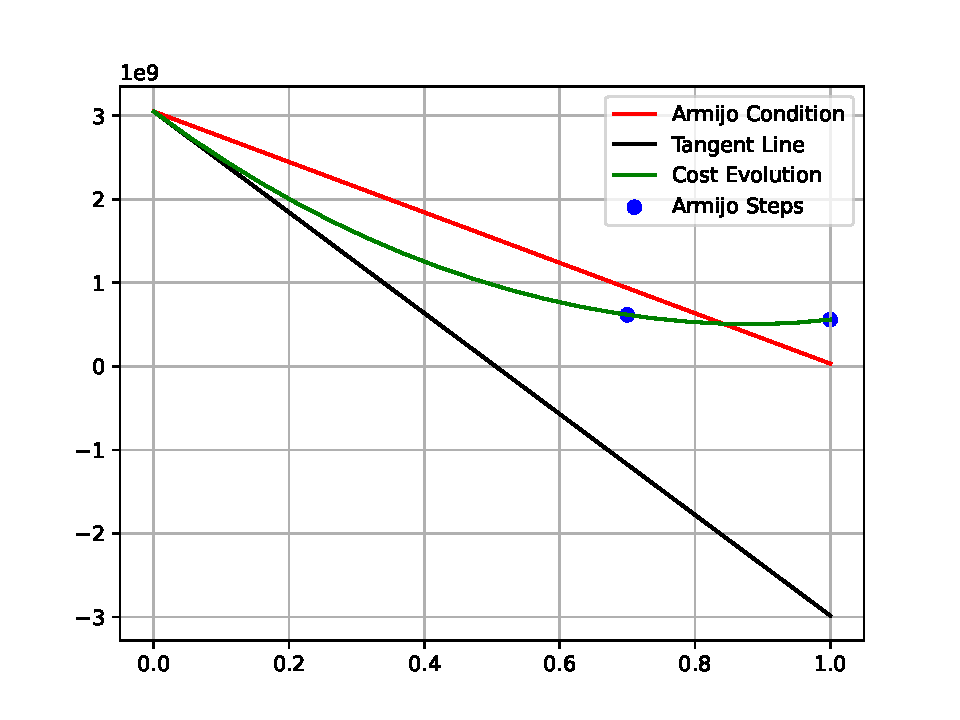
\includegraphics[width=1\linewidth]{img/1-Task1/Armijo_iter_2.pdf}
    \caption{Armijo step-size selection: iteration 2.}
    \label{fig:armijo2}
\end{figure}

\begin{figure}[htb]
    \centering
    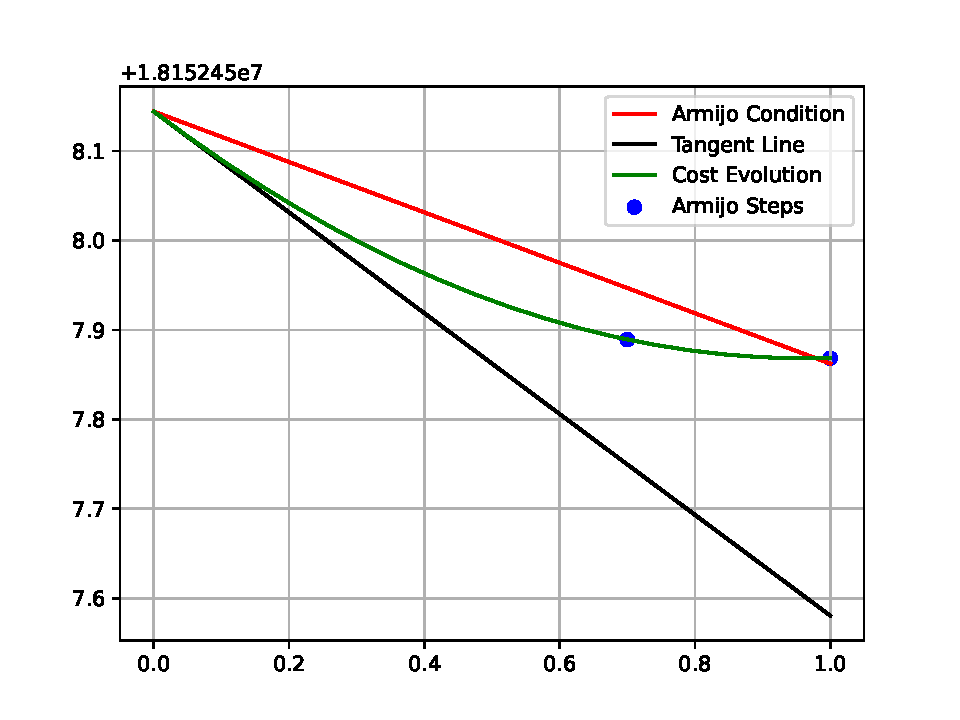
\includegraphics[width=1\linewidth]{img/1-Task1/Armijo_iter_11.pdf}
    \caption{Armijo step-size selection: iteration 11.}
    \label{fig:armijo11}
\end{figure}

\begin{figure}[htb]
    \centering
    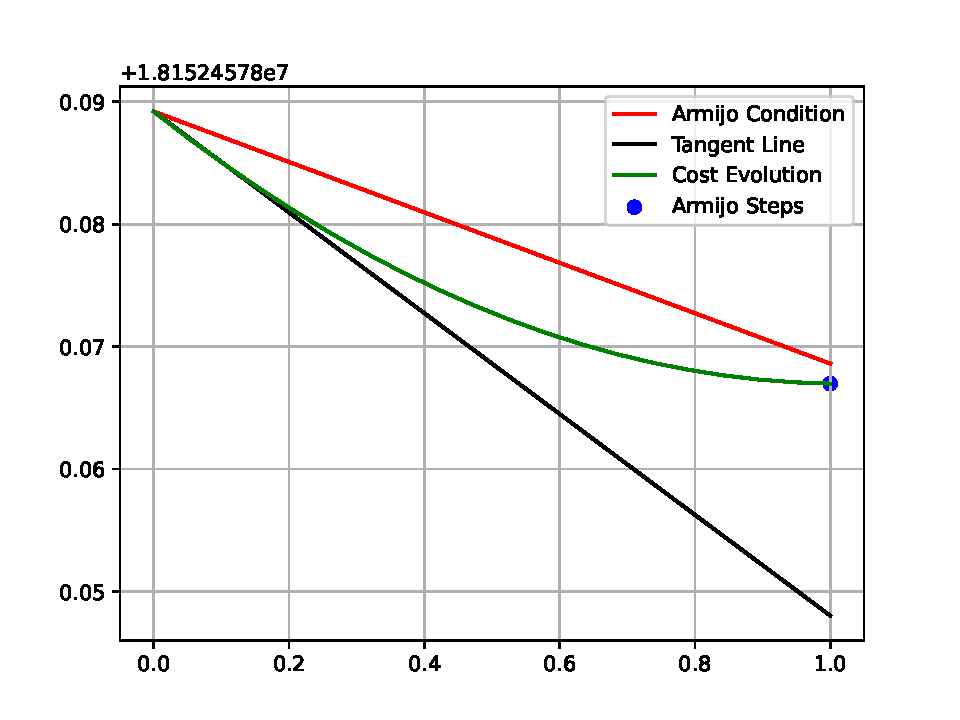
\includegraphics[width=1\linewidth]{img/1-Task1/Armijo_iter_12.pdf}
    \caption{Armijo step-size selection: iteration 12.}
    \label{fig:armijo12}
\end{figure}

\begin{figure}[htb]
    \centering
    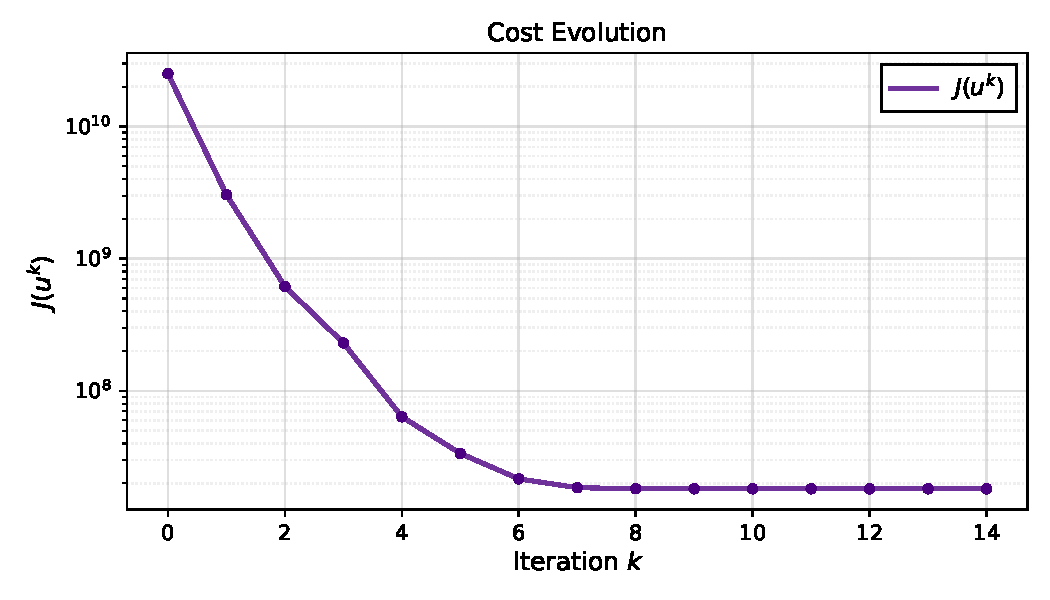
\includegraphics[width=1\linewidth]{img/1-Task1/cost_evolution.pdf}
    \caption{Cost evolution.}
    \label{fig:t1_costevo}
\end{figure}

\begin{figure}[htb]
    \centering
    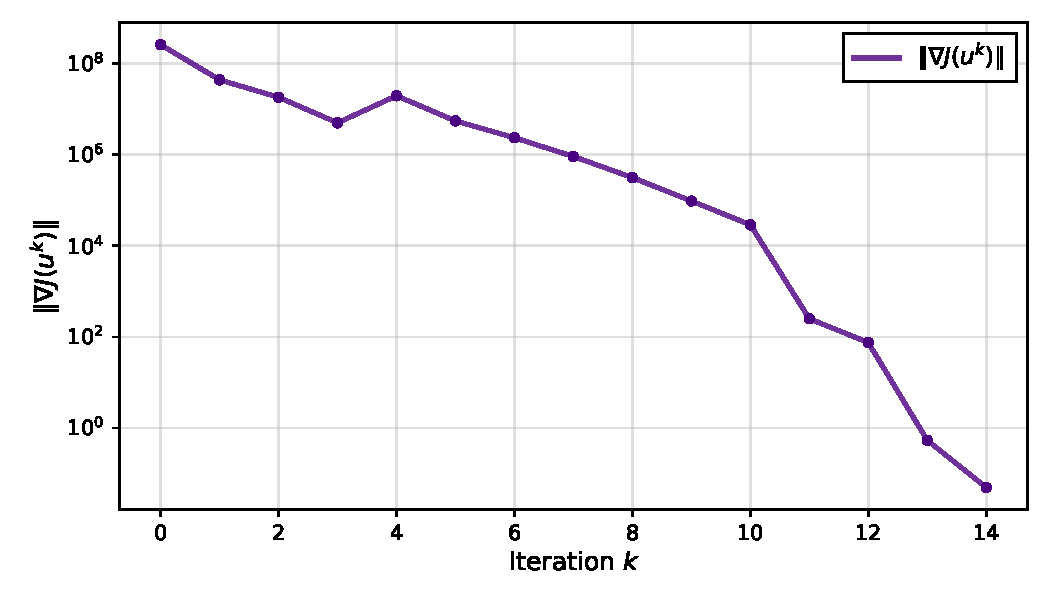
\includegraphics[width=1\linewidth]{img/1-Task1/grad_j_norm.pdf}
    \caption{Cost gradient norm evolution.}
    \label{fig:t1_gradj}
\end{figure}

\begin{figure}[htb]
    \centering
    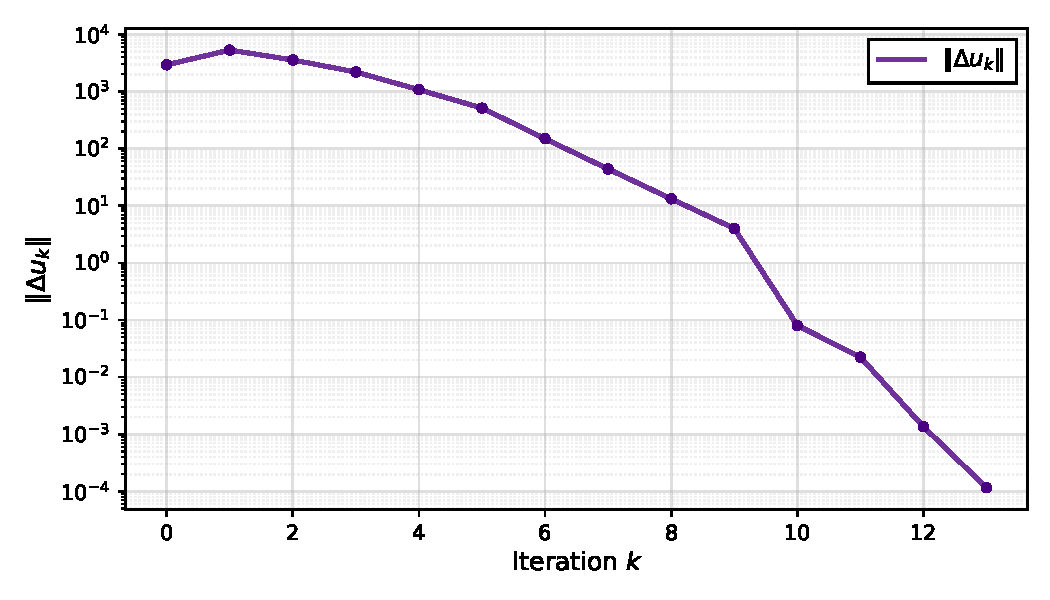
\includegraphics[width=1\linewidth]{img/1-Task1/delta_u_norm.pdf}
    \caption{Evolution of $||\Delta u_k||$.}
    \label{fig:t1_deu}
\end{figure}

\clearpage


\newpage
\section{Constant Cost Matrices Scenario}

The following cost matrices have been adopted:
\begin{equation}
Q_t = Q_T
=
\begin{bmatrix}
    10 & 0 & 0 & 0\\
    0 & 10 & 0 & 0\\
    0 & 0 & 10 & 0\\
    0 & 0 & 0 & 10\\
\end{bmatrix}
\label{eq:CosntantQ}
\end{equation}

\begin{equation}
R_t = 
\begin{bmatrix}
    0.3 & 0 & 0 & 0\\
    0 & 0.3 & 0 & 0\\
    0 & 0 & 0.3 & 0\\
    0 & 0 & 0 & 0.3\\
\end{bmatrix}
\label{eq:ConstantR}
\end{equation}
\newline
Here, a summary of the results is presented.\newline
The performances are obviously worse than the ones presented before.

\begin{figure}[htb]
    \centering
    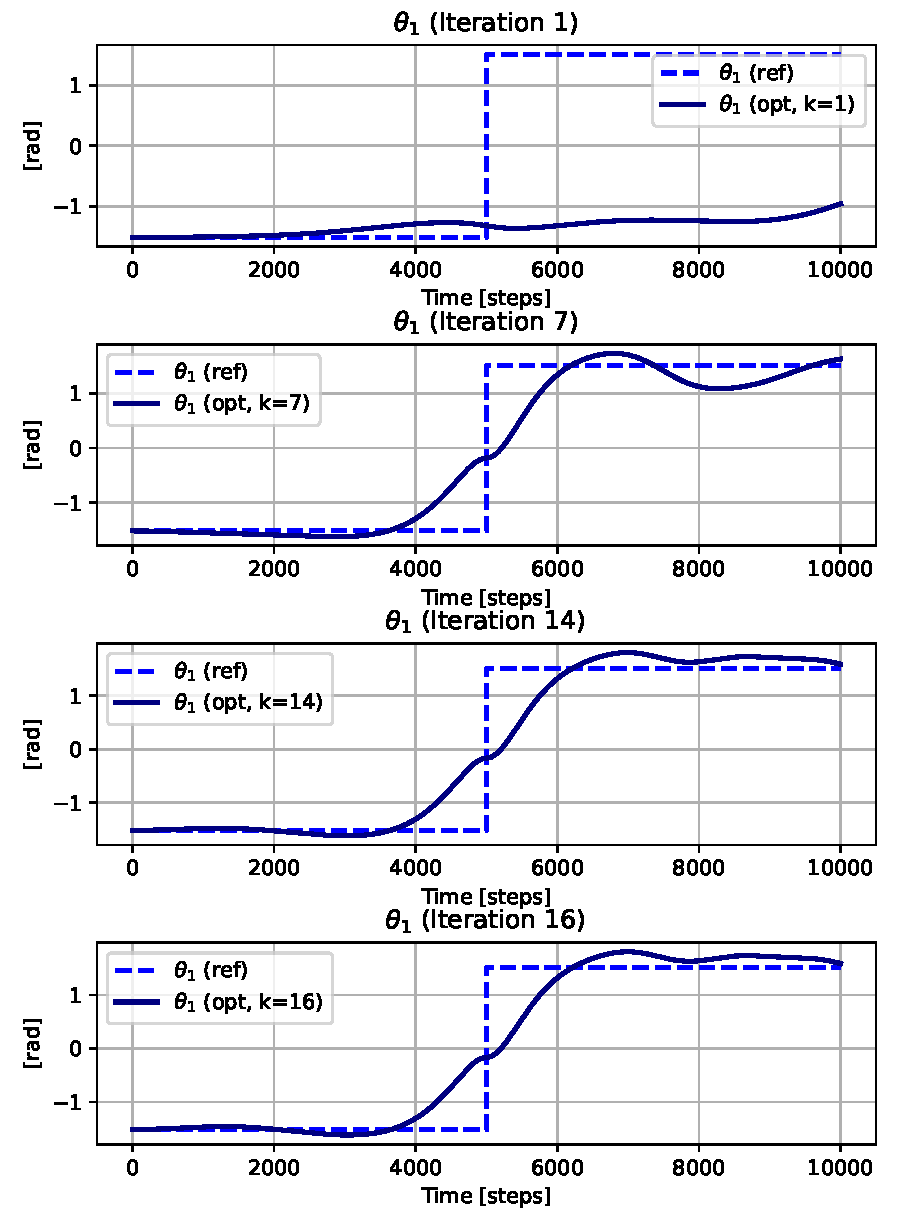
\includegraphics[width=1\linewidth]{img/1-Task1/th1_const.pdf}
    \caption{Evolution of $\theta_1$ with constant Cost Matrices.}
    \label{fig:th1const}
\end{figure}

\begin{figure}[htb]
    \centering
    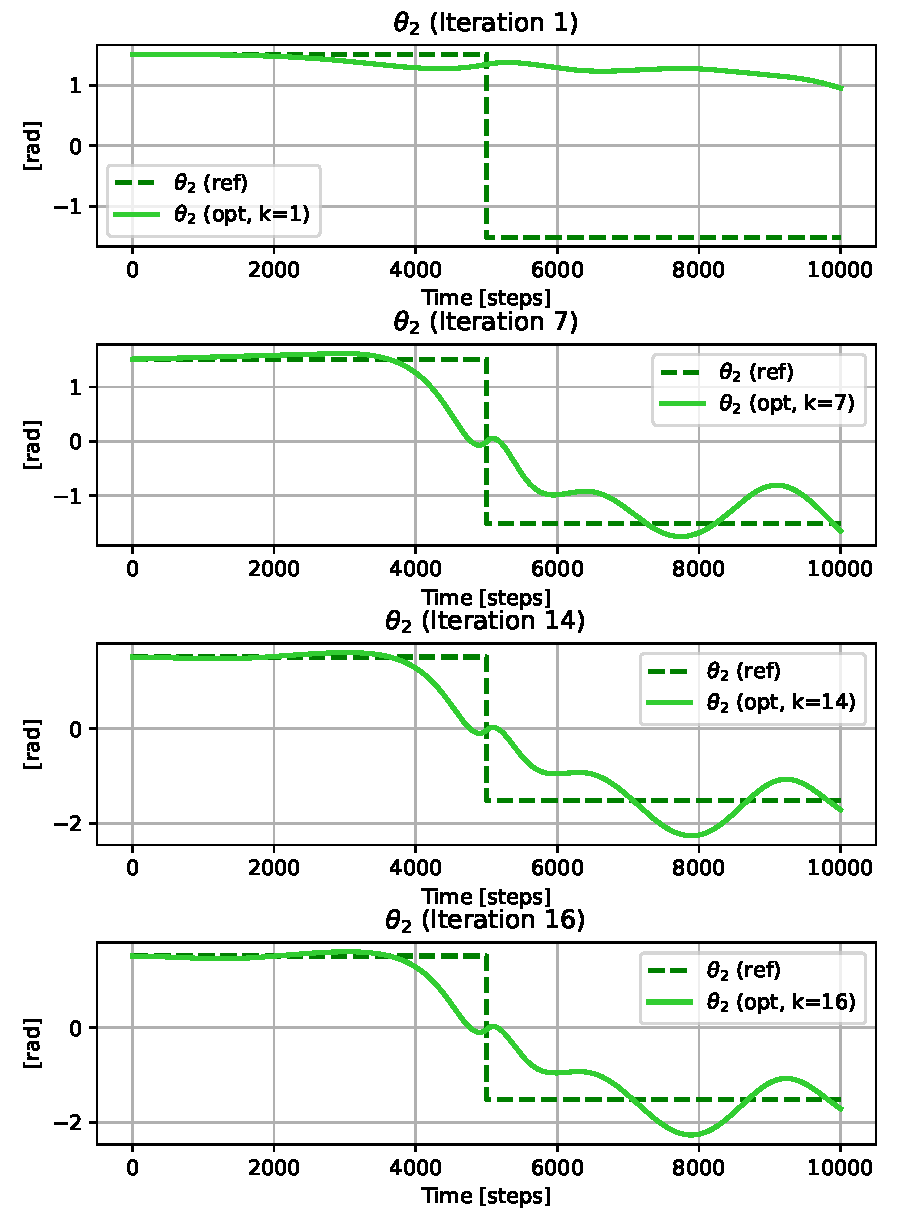
\includegraphics[width=1\linewidth]{img/1-Task1/th2_const.pdf}
    \caption{Evolution of $\theta_2$ with constant Cost Matrices.}
    \label{fig:th2const}
\end{figure}

\clearpage

\begin{figure}[htb]
    \centering
    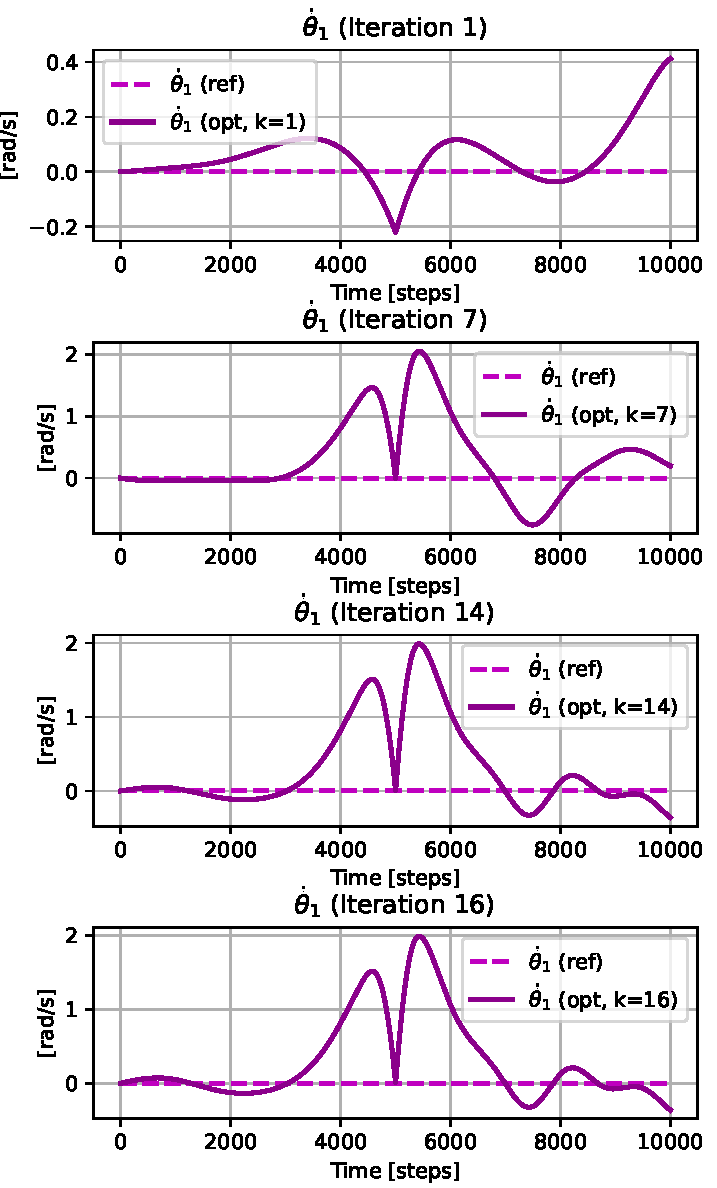
\includegraphics[width=0.9\linewidth]{img/1-Task1/th1dot_const.pdf}
    \caption{Evolution of $\dot{\theta_1}$ with constant Cost Matrices.}
    \label{fig:th1dot_const}
\end{figure}

\begin{figure}[htb]
    \centering
    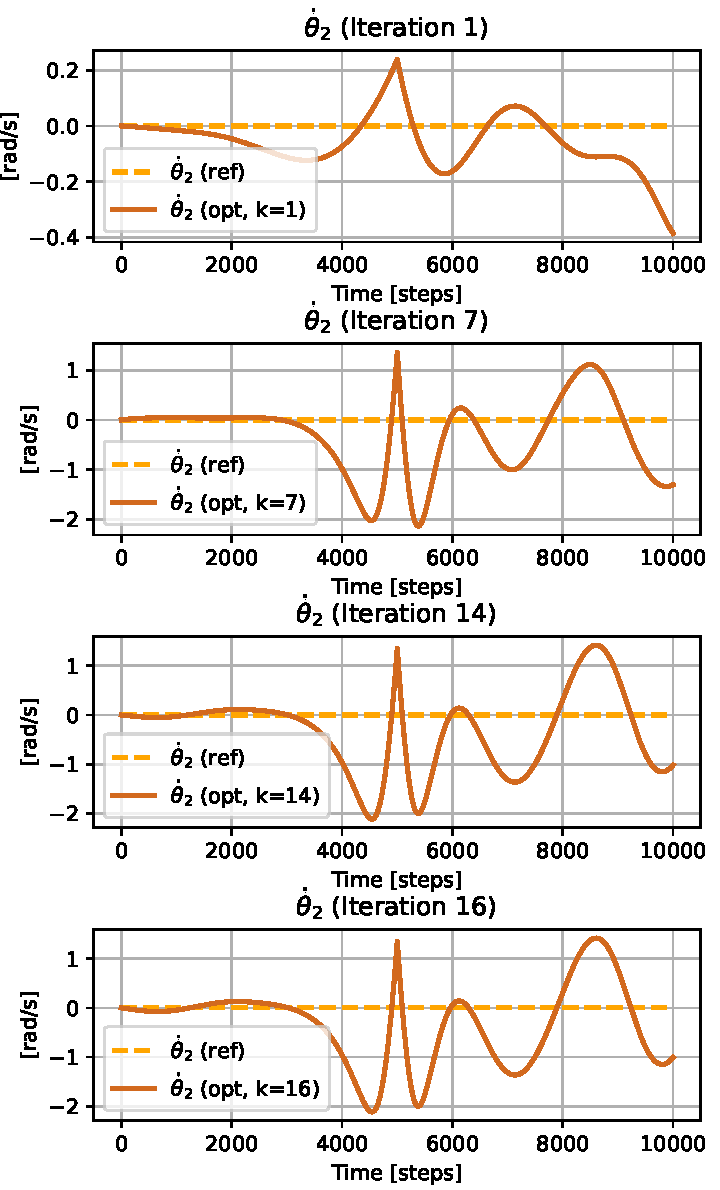
\includegraphics[width=1\linewidth]{img/1-Task1/th2dot_const.pdf}
    \caption{Evolution of $\dot{\theta_2}$ with constant Cost Matrices.}
    \label{fig:th2_const}
\end{figure}

\begin{figure}[htb]
    \centering
    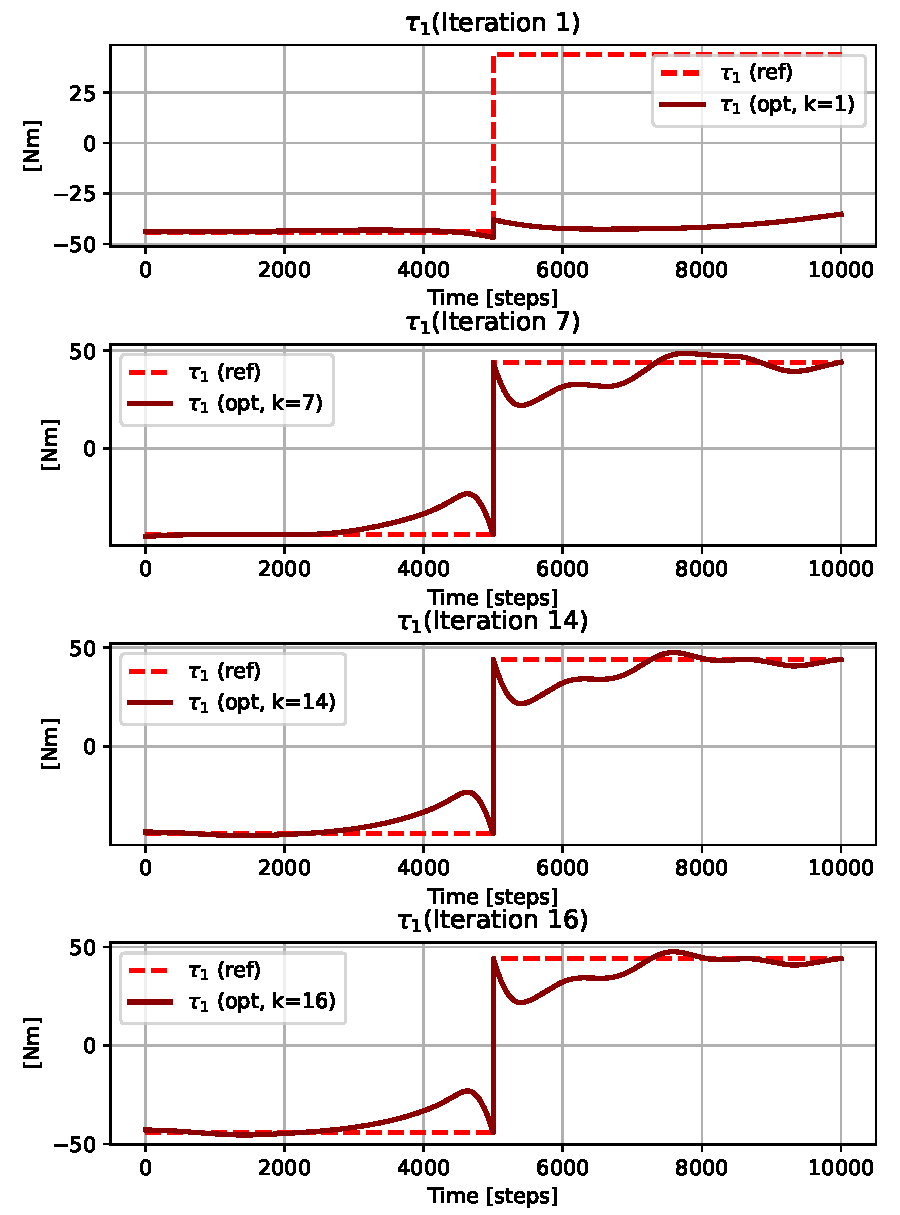
\includegraphics[width=1\linewidth]{img/1-Task1/tau1_const.pdf}
    \caption{Evolution of $\tau$ with constant Cost Matrices.}
    \label{fig:tau_const}
\end{figure}

\clearpage

\begin{figure}[htb]
    \centering
    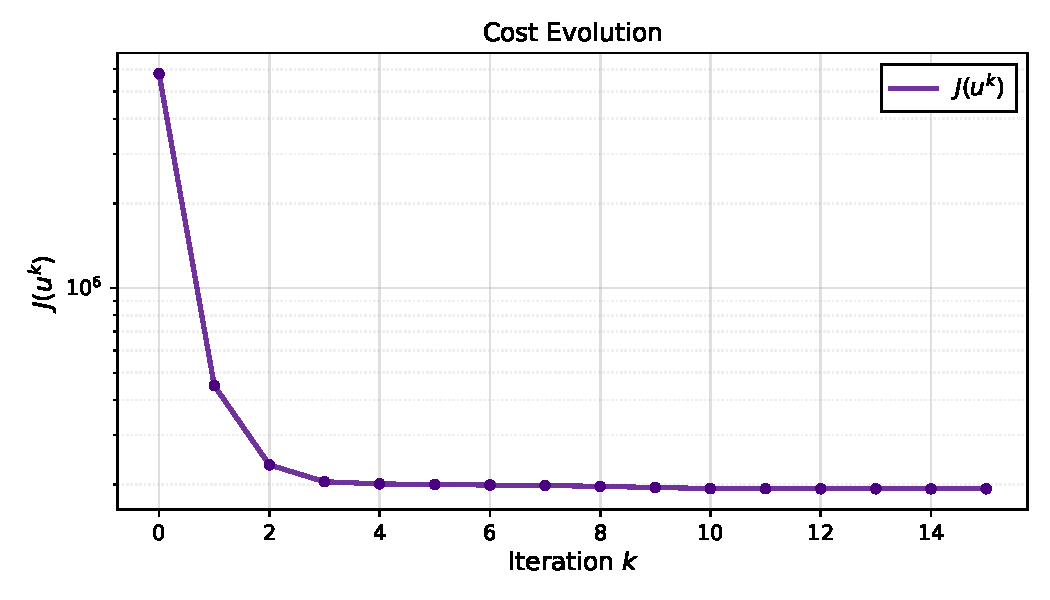
\includegraphics[width=1\linewidth]{img/1-Task1/J_const.pdf}
    \caption{Evolution of cost function with constant Cost Matrices.}
    \label{fig:J_const}
\end{figure}

\begin{figure}[htb]
    \centering
    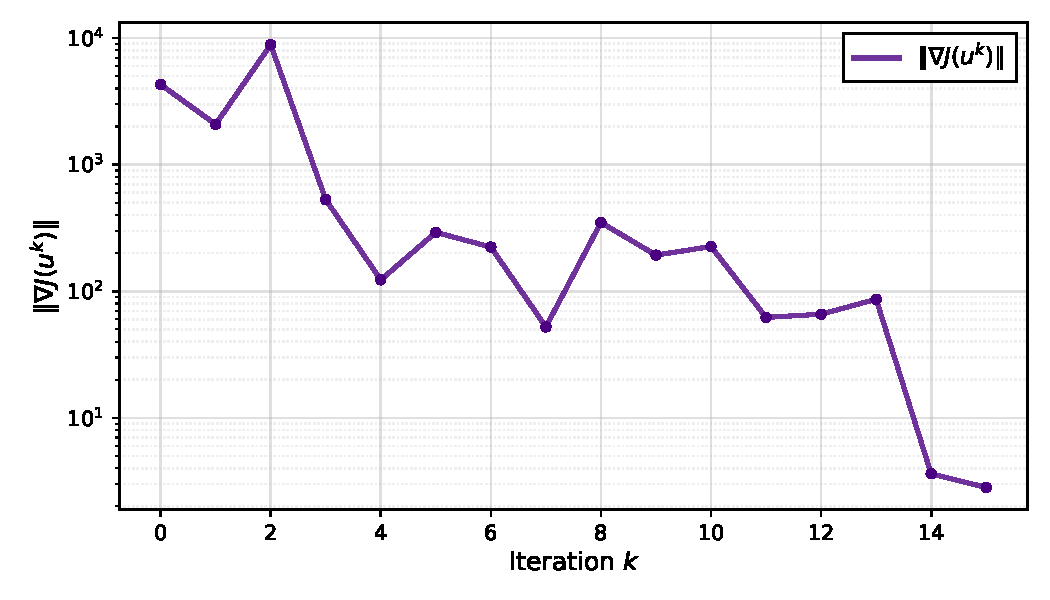
\includegraphics[width=1\linewidth]{img/1-Task1/NormJ_const.pdf}
    \caption{Evolution of $||\nabla J(u)||$ with constant Cost Matrices.}
    \label{fig:NormJ_const}
\end{figure}

\begin{figure}[htb]
    \centering
    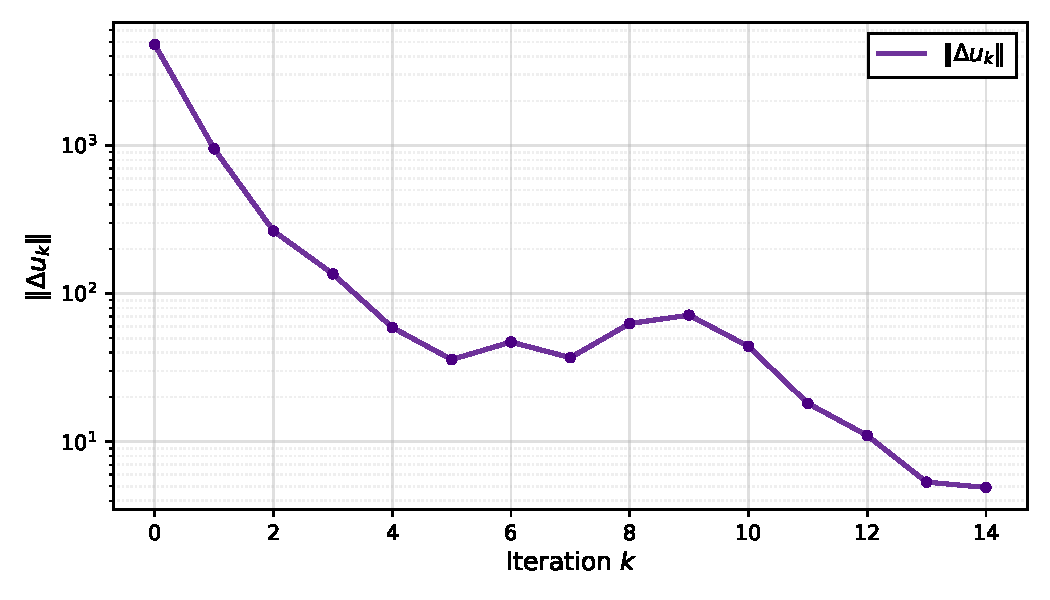
\includegraphics[width=1\linewidth]{img/1-Task1/normdu_const.pdf}
    \caption{Evolution of $||\Delta u_k||$ with constant Cost Matrices.}
    \label{fig:normdu_const}
\end{figure}



% - Required plots:
%   - Optimal trajectory vs. desired reference curve.
%   - Intermediate trajectories.
%   - Armijo descent direction (initial and final iterations).
%   - Norm of descent direction (semi-logarithmic scale).
%   - Cost evolution (semi-logarithmic scale).


